%++++++++++++++++++++++++++++++++++++++++
% Don't modify this section unless you know what you're doing!
\documentclass[letterpaper,11pt]{article}
\usepackage{natbib}
\usepackage[italian]{babel}
\usepackage{float}
\usepackage{subfigure}

\usepackage{listings}
\usepackage[svgnames]{xcolor}
\usepackage{babel,blindtext}
\usepackage{titlesec}

\setcounter{secnumdepth}{4}

\titleformat{\paragraph}
{\normalfont\normalsize\bfseries}{\theparagraph}{1em}{}
\titlespacing*{\paragraph}
{0pt}{3.25ex plus 1ex minus .2ex}{1.5ex plus .2ex}

\lstset{frame=none,
  language=R,
  showstringspaces=false,
  columns=flexible,
  numbers=none,
  basicstyle={\small\ttfamily},
  keywordstyle=\color{Blue},
  stringstyle=\color{Red},
  commentstyle=\color{DarkGreen},
  breaklines=true,
  breakatwhitespace=true,
  moredelim=**[is][\color{blue}]{@}{@},
  tabsize=3}
  
\bibliographystyle{unsrtnat}
\usepackage{tabularx} % extra features for tabular environment
\usepackage{amsmath}  % improve math presentation
\usepackage{graphicx} % takes care of graphic including machinery
\usepackage[margin=1in,letterpaper]{geometry} % decreases margins
%\usepackage{cite} % takes care of citations
\usepackage[final]{hyperref} % adds hyper links inside the generated pdf file
\hypersetup{
	colorlinks=true,       % false: boxed links; true: colored links
	linkcolor=blue,        % color of internal links
	citecolor=blue,        % color of links to bibliography
	filecolor=magenta,     % color of file links
	urlcolor=blue         
}
%+++++++++++++++++++++++++++++++++++++++
\begin{document}

\title{Machine Learning Project \\\textbf{Customer Personality Analysis}}
%\author{Mario Avolio}

\author{
  Mario Avolio\\
  \texttt{880995}
  \and
  Rocco Gianni Rapisarda\\
  \texttt{845197}
}
\date{\today}
\maketitle

\begin{abstract}
L'apprendimento automatico e la statistica sono discipline strettamente collegate. Secondo \href{https://en.wikipedia.org/wiki/Michael\_I.\_Jordan}{Michael I. Jordan}, le idee dell'apprendimento automatico, dai principi metodologici agli strumenti teorici, sono stati sviluppati prima in statistica. In questo elaborato si riporta l'attività di sviluppo e sperimentazione di diversi modelli di \textbf{Machine Learning} per l'analisi approfondita dei clienti ideali per una generica azienda. La concentrazione è stata focalizzata soprattutto sul \textbf{Clustering} mediante l'algoritmo \textbf{K-Means}, sebbene nel corso della trattazione si esporranno anche altre metodologie utilizzate per l'analisi dei dati.
\end{abstract}

\section{Descrizione del dominio di riferimento e obiettivi dell’elaborato}
Molto spesso lo sviluppo di nuovi prodotti o servizi è attivato dall’imitazione dei concorrenti e da analisi di mercato generiche, mentre al cliente si dedica poca attenzione. L’acquisto è prima di tutto un’esperienza ed è necessario comprendere quali bisogni la guidano: solo così ogni segmento di mercato individuato sarà connesso con la capacità dell’azienda di soddisfare le aspettative dei clienti, comprese quelle inespresse. Progettare, sviluppare e vendere prodotti non connessi con il proprio target rappresenta un costo insostenibile, mentre è necessario progettare uno sviluppo in linea con la \textit{customer satisfaction}. Per questo motivo \href{https://www.kaggle.com/imakash3011/customer-personality-analysis}{Customer Personality Analysis} riguarda un'analisi dettagliata dei clienti ideali per una generica azienda. Il compito fondamentale è quello di aiutare un'attività commerciale a comprendere meglio i propri compratori al fine di rendere più semplice la modifica e la scelta dei propri prodotti, in relazione alle esigenze richieste dagli acquirenti. L'obiettivo che ha spinto ad analizzare questo insieme di dati è inerente alle \textbf{diverse} personalità e comportamenti che gli acquirenti assumono durante il ruolo di potenziali clienti aziendali. Per questo motivo le aziende non possono adottare lo stesso approccio per ogni tipologia di plausibile compratore. 

\section{Scelte di design, ipotesi e assunzioni}
TODO

\section{Descrizione del training set}
\subsection{Attributi}
Si fornisce la descrizione originale degli attributi analizzati.
\subsubsection*{People}
\begin{itemize}
    \item ID: Customer's unique identifier
    \item Year\_Birth: Customer's birth year
    \item Education: Customer's education level
    \item Marital\_Status: Customer's marital status
    \item Income: Customer's yearly household income
    \item Kidhome: Number of children in customer's household
    \item Teenhome: Number of teenagers in customer's household
    \item Dt\_Customer: Date of customer's enrollment with the company
    \item Recency: Number of days since customer's last purchase
    \item Complain: 1 if the customer complained in the last 2 years, 0 otherwise
\end{itemize}


\subsubsection*{Products}
\begin{itemize}
\item MntWines: Amount spent on wine in last 2 years
\item MntFruits: Amount spent on fruits in last 2 years
\item MntMeatProducts: Amount spent on meat in last 2 years
\item MntFishProducts: Amount spent on fish in last 2 years
\item MntSweetProducts: Amount spent on sweets in last 2 years
\item MntGoldProds: Amount spent on gold in last 2 years
\end{itemize}

\subsubsection*{Promotion}
\begin{itemize}
\item NumDealsPurchases: Number of purchases made with a discount
\item AcceptedCmp1: 1 if customer accepted the offer in the 1st campaign, 0 otherwise
\item AcceptedCmp2: 1 if customer accepted the offer in the 2nd campaign, 0 otherwise
\item AcceptedCmp3: 1 if customer accepted the offer in the 3rd campaign, 0 otherwise
\item AcceptedCmp4: 1 if customer accepted the offer in the 4th campaign, 0 otherwise
\item AcceptedCmp5: 1 if customer accepted the offer in the 5th campaign, 0 otherwise
 \item Response: 1 if customer accepted the offer in the last campaign, 0 otherwise
\end{itemize}

\subsubsection*{Place}
\begin{itemize}
\item NumWebPurchases: Number of purchases made through the company’s website
\item NumCatalogPurchases: Number of purchases made using a catalogue
\item NumStorePurchases: Number of purchases made directly in stores
\item NumWebVisitsMonth: Number of visits to company’s website in the last month
\end{itemize}
La tabella \ref{fig:sapply(customers, class)} fornisce un'iniziale descrizione della tipologia di variabili presenti nel dataset. \\
\begin{table}[h!t]
\centering
\begin{tabular}{rl}
  \hline
 & sapply(customers, class) \\ 
  \hline
ID & integer \\ 
  Year\_Birth & integer \\ 
  Education & character \\ 
  Marital\_Status & character \\ 
  Income & integer \\ 
  Kidhome & integer \\ 
  Teenhome & integer \\ 
  Dt\_Customer & character \\ 
  Recency & integer \\ 
  MntWines & integer \\ 
  MntFruits & integer \\ 
  MntMeatProducts & integer \\ 
  MntFishProducts & integer \\ 
  MntSweetProducts & integer \\ 
  MntGoldProds & integer \\ 
  NumDealsPurchases & integer \\ 
  NumWebPurchases & integer \\ 
  NumCatalogPurchases & integer \\ 
  NumStorePurchases & integer \\ 
  NumWebVisitsMonth & integer \\ 
  AcceptedCmp3 & integer \\ 
  AcceptedCmp4 & integer \\ 
  AcceptedCmp5 & integer \\ 
  AcceptedCmp1 & integer \\ 
  AcceptedCmp2 & integer \\ 
  Complain & integer \\ 
  Z\_CostContact & integer \\ 
  Z\_Revenue & integer \\ 
  Response & integer \\ 
   \hline
\end{tabular}
\caption{Output funzione \textit{sapply(customers, class)}}
\label{fig:sapply(customers, class)}
\end{table}
\subsection{Prime analisi}
Prima di fornire un'analisi dettagliata degli elementi del dataset si è ritenuto necessario effettuare una prima ispezione di alto livello, senza entrare nel dettaglio di ciascun attributo. Il dataset viene importato mediante la funzione:
\begin{lstlisting}[language=R]
customers <- read.csv(paste(getwd(),"/Data/marketing_campaign.csv",sep = ""), header=TRUE, sep="\t",  stringsAsFactors=F) # use TAB as separator!
\end{lstlisting}
\begin{figure}[H]
     \begin{center}
%
        \subfigure[BoxPlot Year\_Birth]{%

            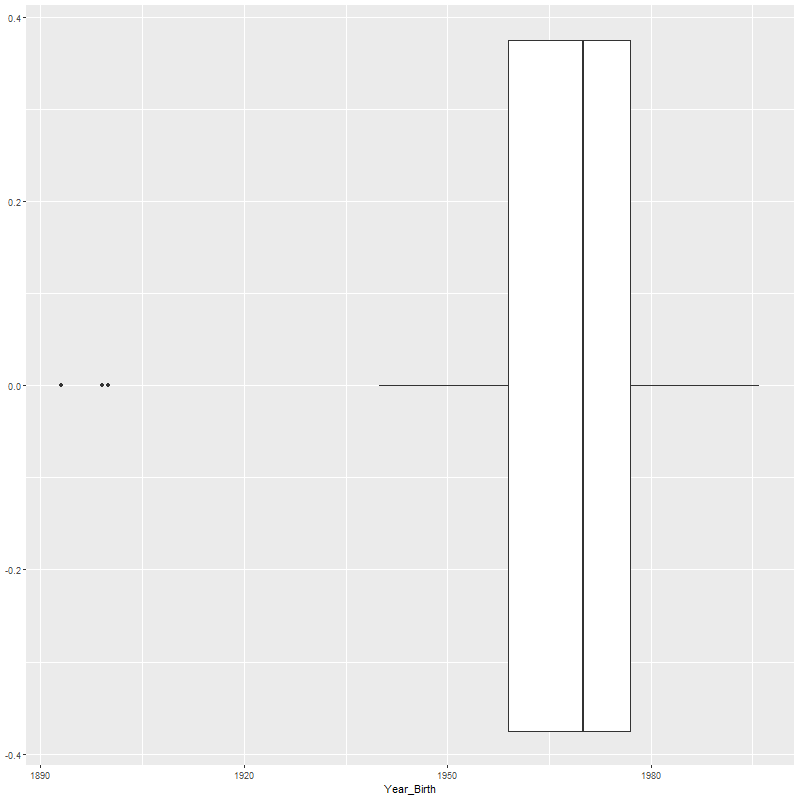
\includegraphics[width=0.4\textwidth]{Img/DESCRIPTION/DESCRIPTION001.png}
        }%
        \subfigure[BoxPlot Income]{%
            \label{fig:Histogram_Income}
            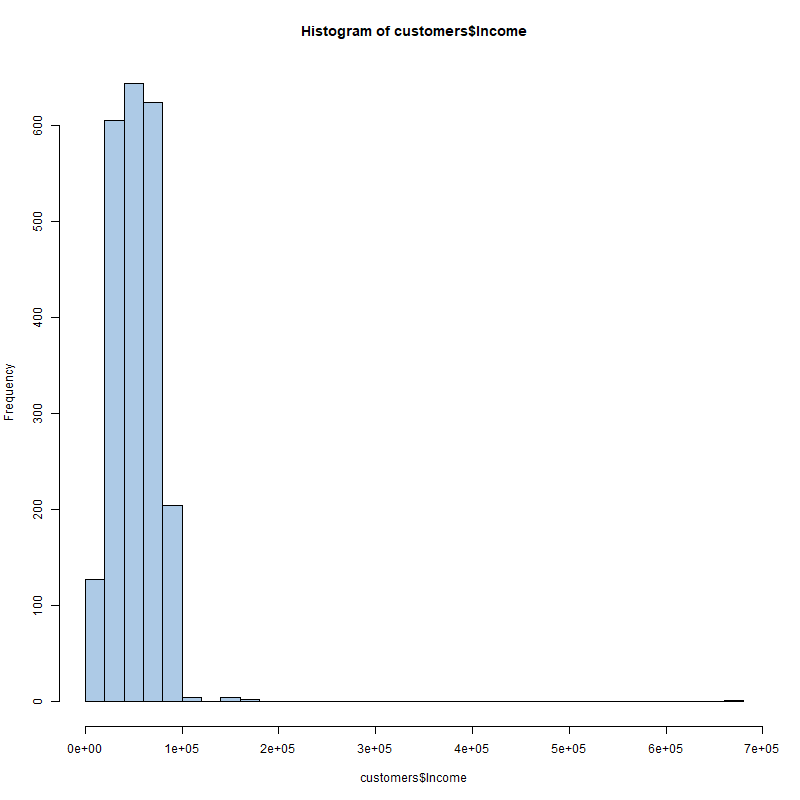
\includegraphics[width=0.4\textwidth]{Img/DESCRIPTION/DESCRIPTION020.png}
        }\\ %  ------- End of the first row ----------------------%
        \subfigure[BoxPlot KidHome]{%

            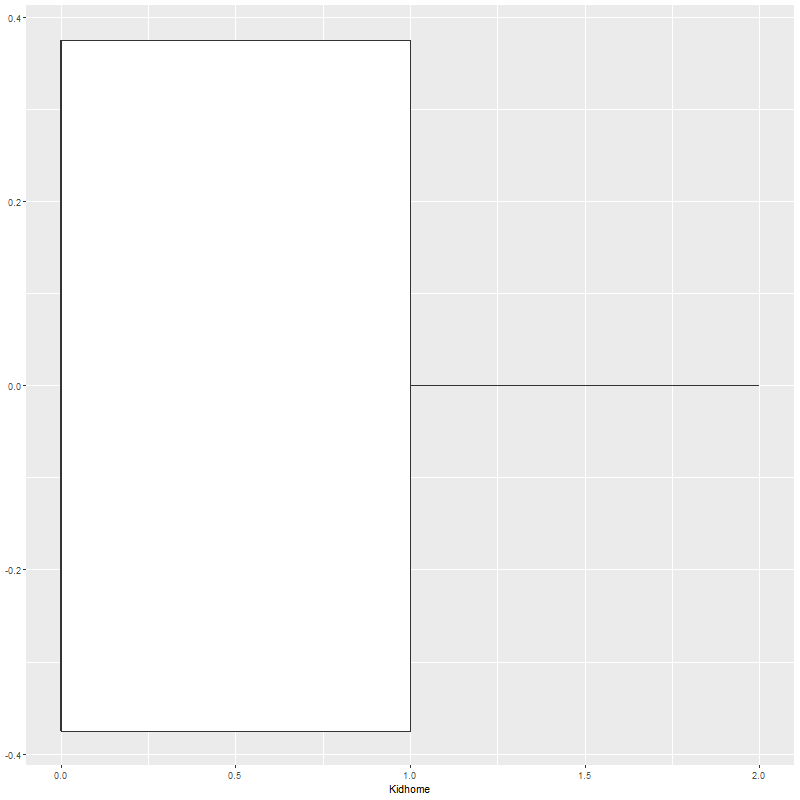
\includegraphics[width=0.4\textwidth]{Img/DESCRIPTION/DESCRIPTION004.png}
        }%
%
    \end{center}
\end{figure}
\begin{figure}[H]
     \begin{center}
%
        \subfigure[BoxPlot TeenHome]{%

            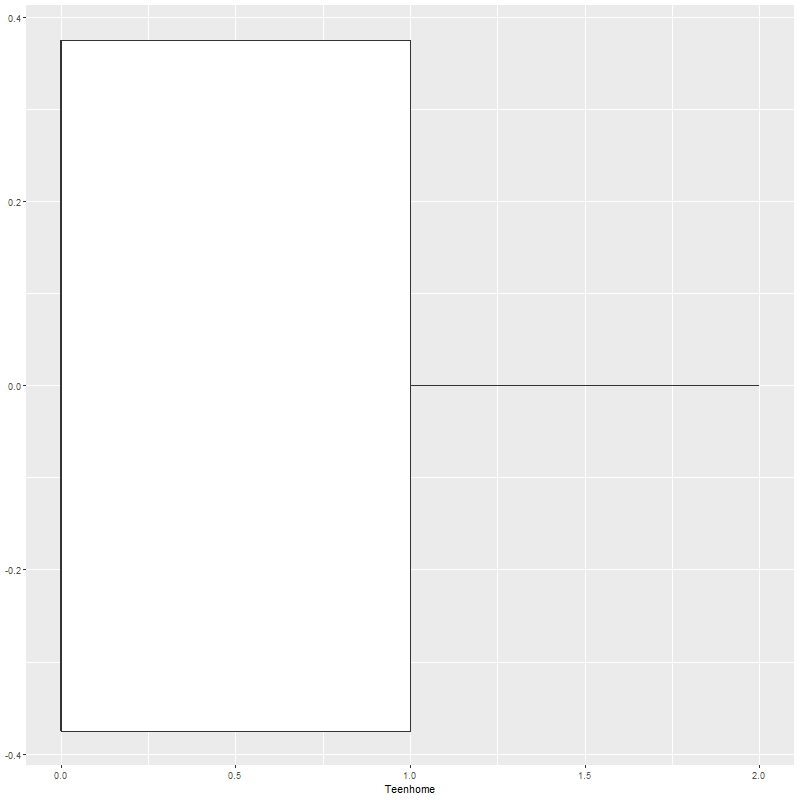
\includegraphics[width=0.4\textwidth]{Img/DESCRIPTION/DESCRIPTION005.png}
        }%
        \subfigure[BoxPlot Recency]{%

           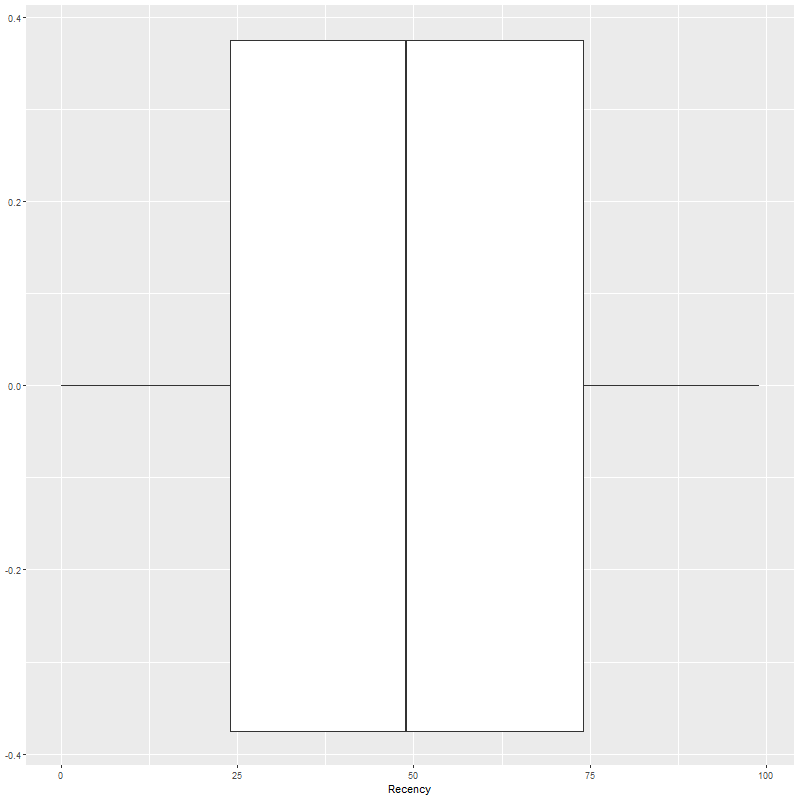
\includegraphics[width=0.4\textwidth]{Img/DESCRIPTION/DESCRIPTION006.png}
        }\\ %  ------- End of the first row ----------------------%
        \subfigure[BoxPlot MntWines]{%

            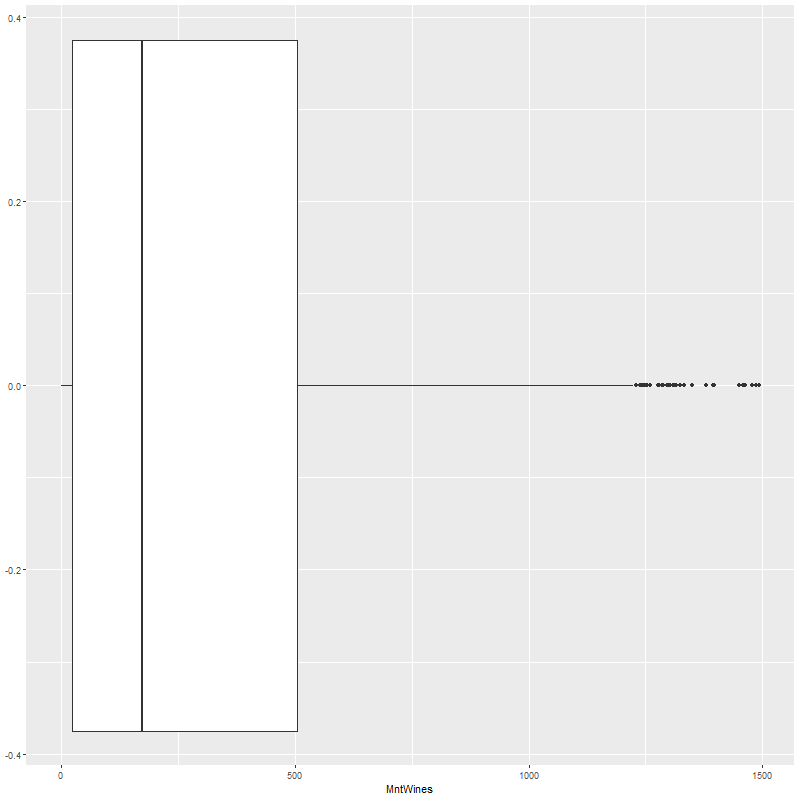
\includegraphics[width=0.4\textwidth]{Img/DESCRIPTION/DESCRIPTION007.png}
        }%
        \subfigure[BoxPlot MntFruits]{%

            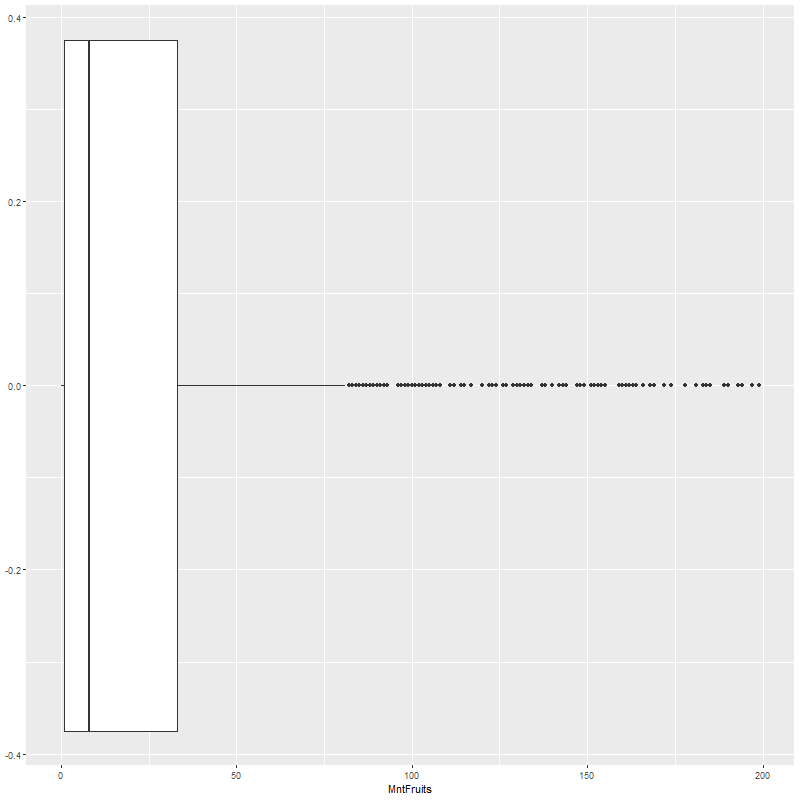
\includegraphics[width=0.4\textwidth]{Img/DESCRIPTION/DESCRIPTION008.png}
        }%
%
    \end{center}
\end{figure}
\begin{figure}[H]
     \begin{center}
%
        \subfigure[BoxPlot MntMeatProducts]{%

            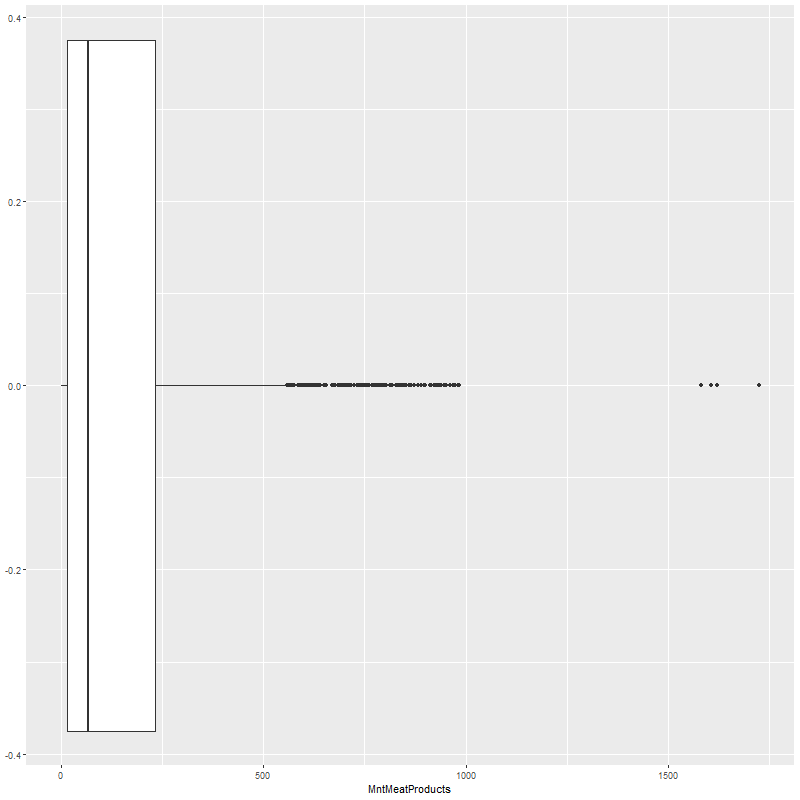
\includegraphics[width=0.4\textwidth]{Img/DESCRIPTION/DESCRIPTION009.png}
        }%
        \subfigure[BoxPlot MntFishProducts]{%

           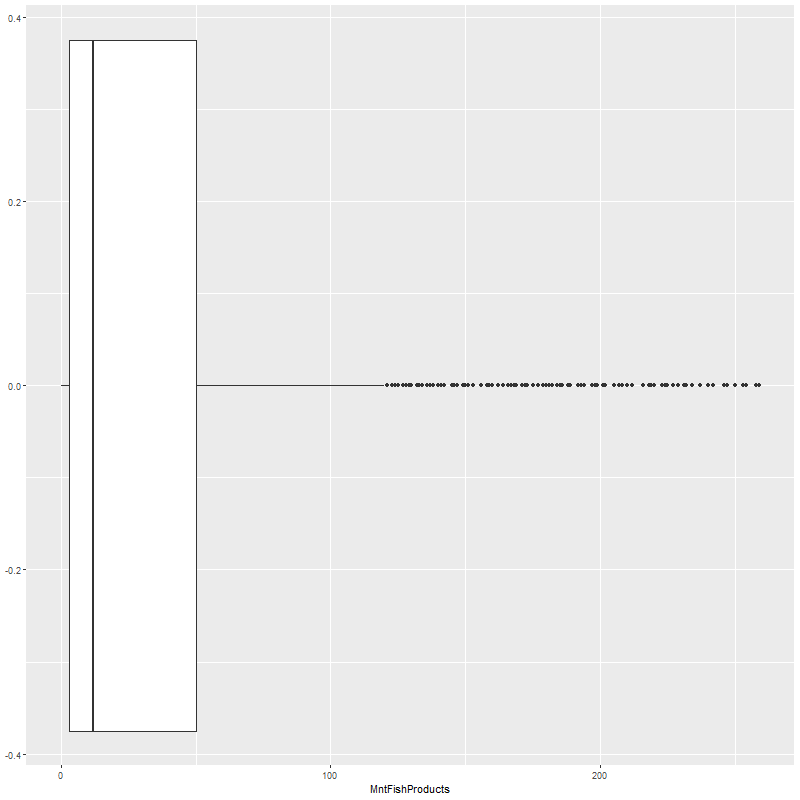
\includegraphics[width=0.4\textwidth]{Img/DESCRIPTION/DESCRIPTION010.png}
        }\\ %  ------- End of the first row ----------------------%
        \subfigure[BoxPlot MntSweetProducts]{%

            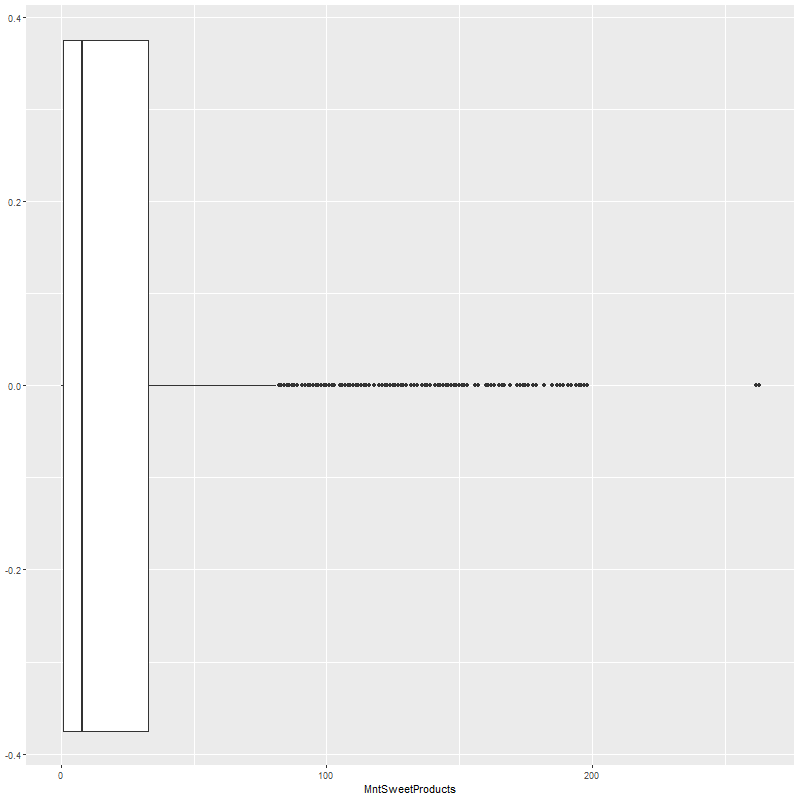
\includegraphics[width=0.4\textwidth]{Img/DESCRIPTION/DESCRIPTION011.png}
        }%
        \subfigure[BoxPlot MntGoldProds]{%

            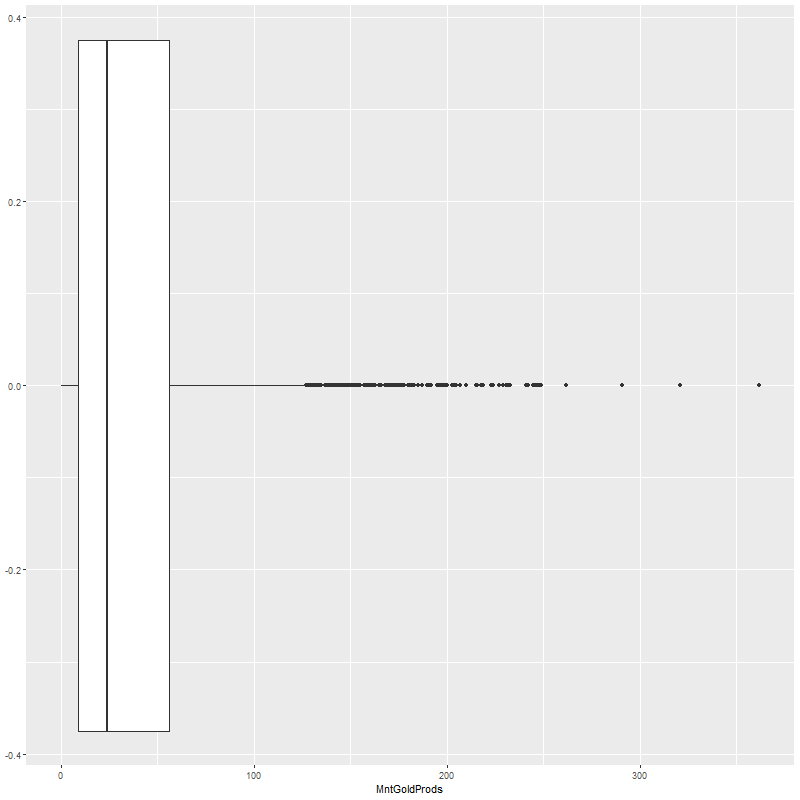
\includegraphics[width=0.4\textwidth]{Img/DESCRIPTION/DESCRIPTION012.png}
        }%
%
    \end{center}
\end{figure}
\begin{figure}[H]
     \begin{center}
%
        \subfigure[BoxPlot numDealsPurchases]{%

            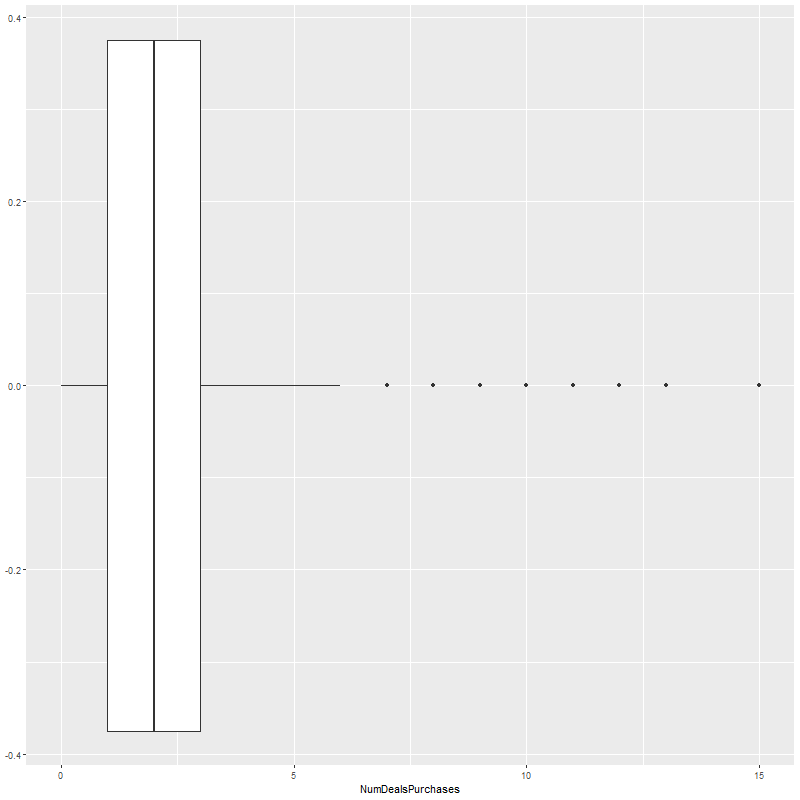
\includegraphics[width=0.4\textwidth]{Img/DESCRIPTION/DESCRIPTION013.png}
        }%
        \subfigure[BoxPlot NumWebPurchases]{%

           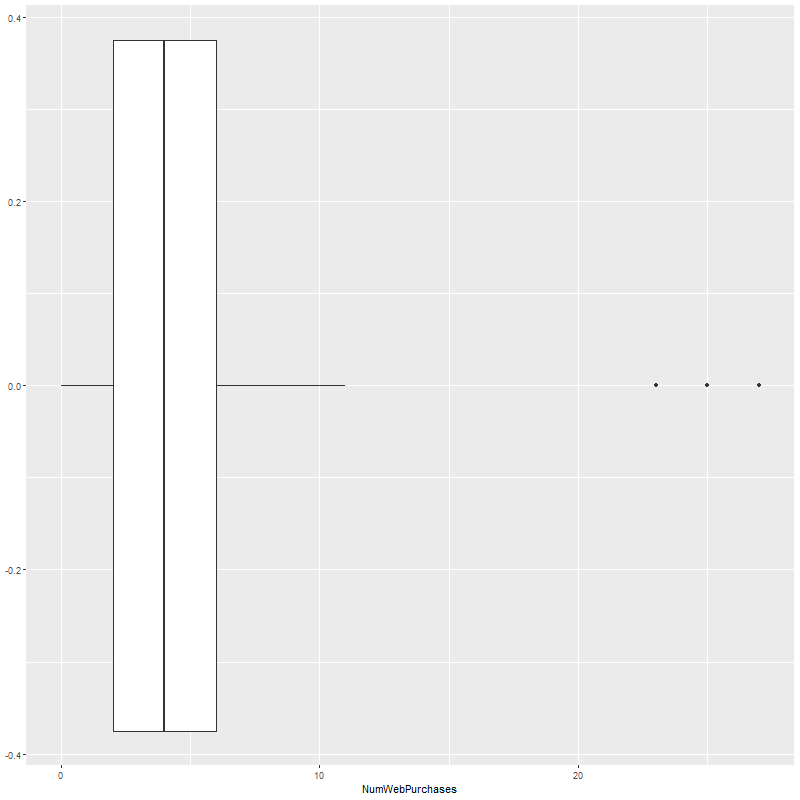
\includegraphics[width=0.4\textwidth]{Img/DESCRIPTION/DESCRIPTION014.png}
        }\\ %  ------- End of the first row ----------------------%
        \subfigure[BoxPlot NumCatalogPurchases]{%

            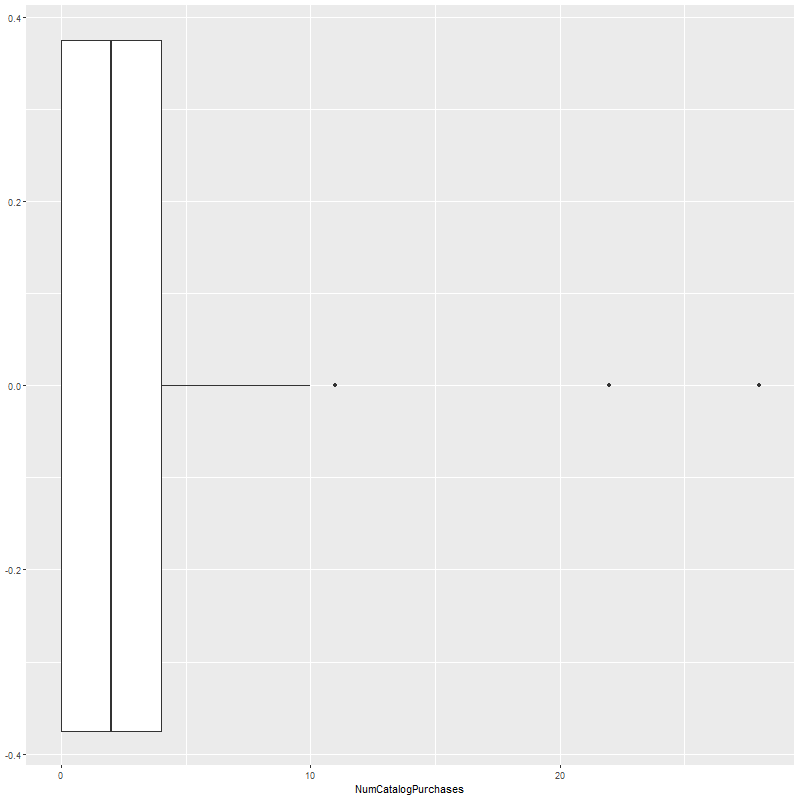
\includegraphics[width=0.4\textwidth]{Img/DESCRIPTION/DESCRIPTION015.png}
        }%
        \subfigure[BoxPlot NumStorePurchases]{%

            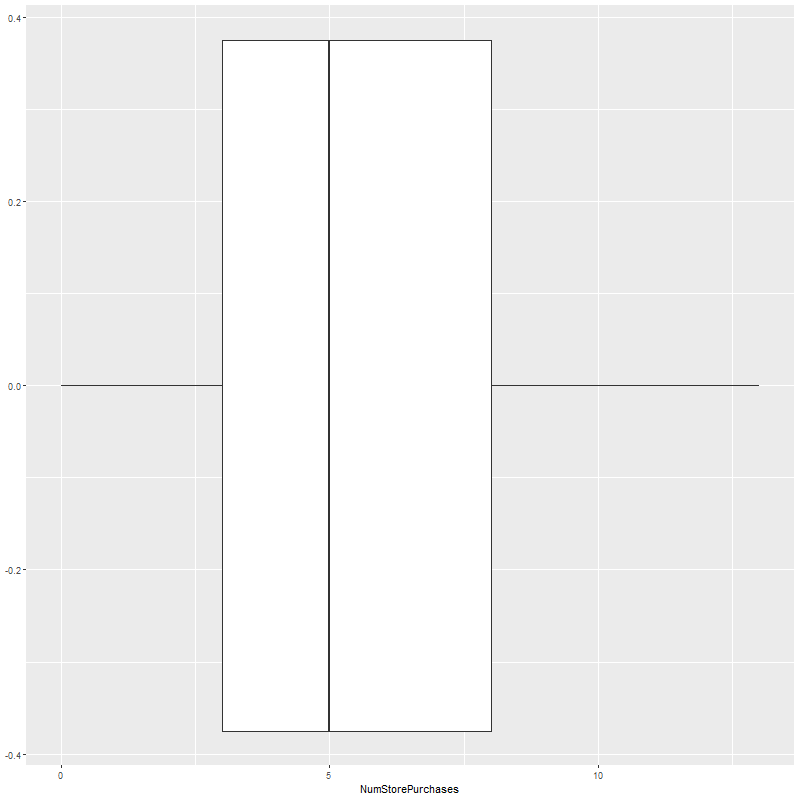
\includegraphics[width=0.4\textwidth]{Img/DESCRIPTION/DESCRIPTION016.png}
        }%
%
    \end{center}
\end{figure}
\begin{figure}[H]
     \begin{center}
%
        \subfigure[BoxPlot NumDealsPurchases]{%

            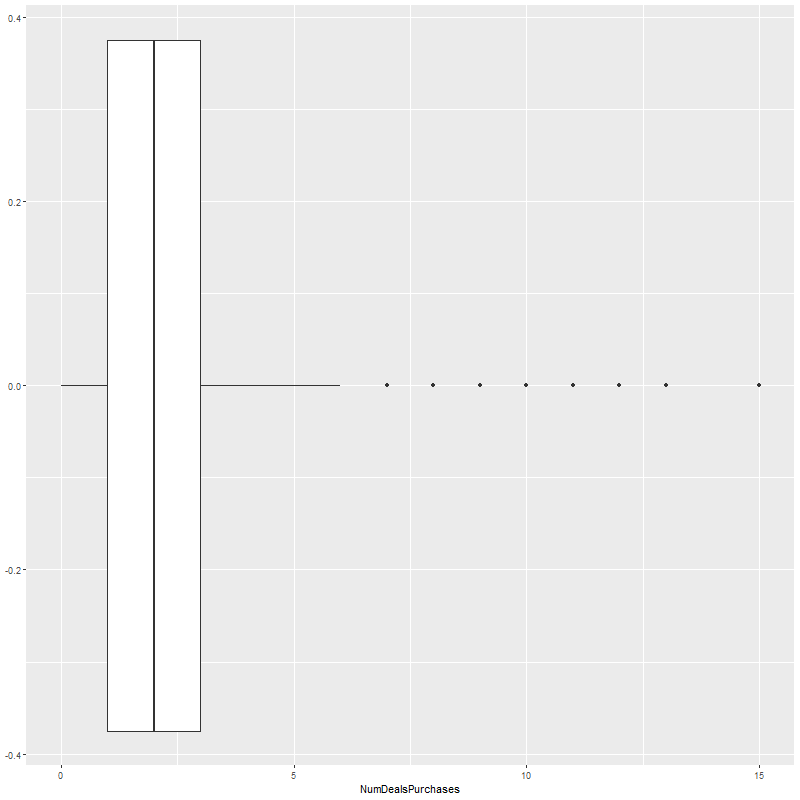
\includegraphics[width=0.4\textwidth]{Img/DESCRIPTION/DESCRIPTION017.png}
        }%
        \subfigure[BoxPlot Z\_CostContact]{%
            \label{fig:Z_Revenue}
           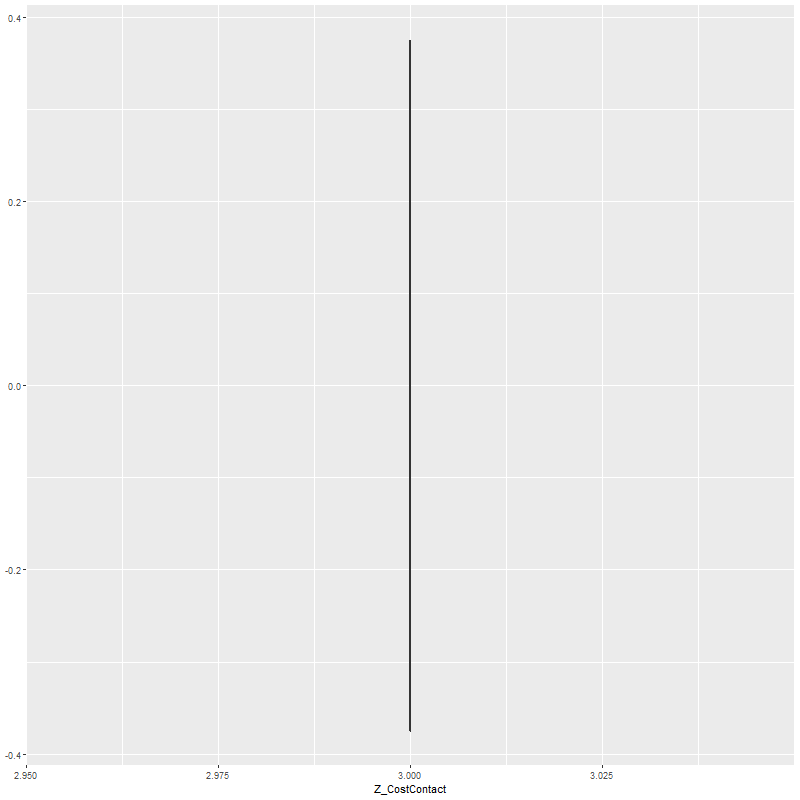
\includegraphics[width=0.4\textwidth]{Img/DESCRIPTION/DESCRIPTION018.png}
        }\\ %  ------- End of the first row ----------------------%
        \subfigure[BoxPlot Z\_Revenue]{%
            \label{fig:Z_CostContact}
            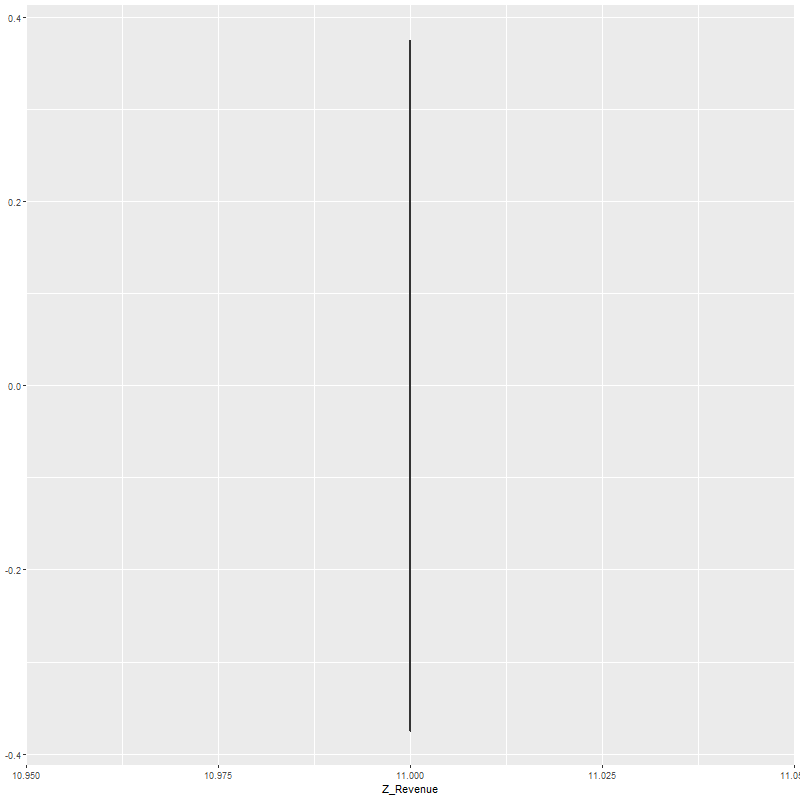
\includegraphics[width=0.4\textwidth]{Img/DESCRIPTION/DESCRIPTION019.png}
        }%
        \subfigure[BoxPlot Income]{%
            \label{fig:BoxPlot_Income}
            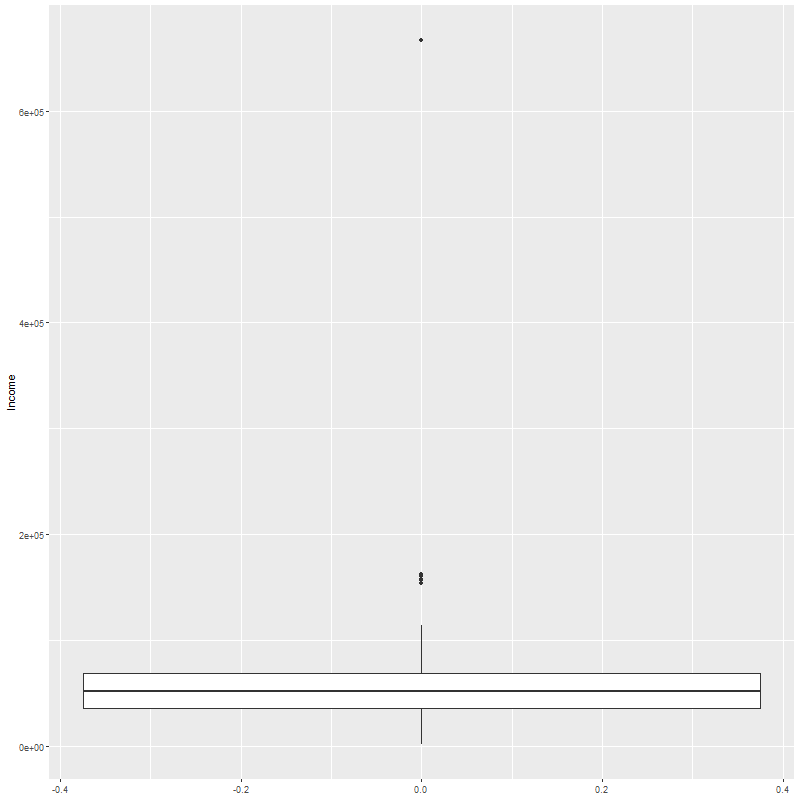
\includegraphics[width=0.4\textwidth]{Img/DESCRIPTION/DESCRIPTION021.png}
        }%
%
    \end{center}
\end{figure}
Durante questa prima indagine sono stati effettuati controlli di base sulle variabili. In particolare, dalle analisi dei boxplot riportati rispettivamente nelle figure \ref{fig:Z_CostContact} e \ref{fig:Z_Revenue} è doveroso notare la mancanza di \textbf{varianza} di tali variabili, questo aspetto sarà successivamente preso in considerazione durante la fase di preprocessing.\\ Inoltre durante l'analisi delle figure \ref{fig:BoxPlot_Income} e \ref{fig:Histogram_Income}, mediante un apposito \textit{warning} durante l'esecuzione del codice R, si è notata la presenza di alcuni valori mancanti.
\begin{lstlisting}[language=R]
hist(customers$Income,40,col="#adcae6")
ggplot(customers, aes(y = Income)) + geom_boxplot()
n_miss(customers) # counting the total number of missing values in the data
miss_var_summary(customers) # Summarizing missingness in each variable 
\end{lstlisting}
La tabella \ref{fig:miss_var_summary(customers)} mostra l'output del comando \textit{miss\_var\_summary(customers)}, dove si possono notare 24 valori mancanti nella variabile \textit{Income}.
\begin{table}[h!t]
\centering
\begin{tabular}{rlrr}
  \hline
 & variable & n\_miss & pct\_miss \\ 
  \hline
1 & Income &  24 & 1.07 \\ 
  2 & ID &   0 & 0.00 \\ 
  3 & Year\_Birth &   0 & 0.00 \\ 
  4 & Education &   0 & 0.00 \\ 
  5 & Marital\_Status &   0 & 0.00 \\ 
  6 & Kidhome &   0 & 0.00 \\ 
  7 & Teenhome &   0 & 0.00 \\ 
  8 & Dt\_Customer &   0 & 0.00 \\ 
  9 & Recency &   0 & 0.00 \\ 
  10 & MntWines &   0 & 0.00 \\ 
  11 & MntFruits &   0 & 0.00 \\ 
  12 & MntMeatProducts &   0 & 0.00 \\ 
  13 & MntFishProducts &   0 & 0.00 \\ 
  14 & MntSweetProducts &   0 & 0.00 \\ 
  15 & MntGoldProds &   0 & 0.00 \\ 
  16 & NumDealsPurchases &   0 & 0.00 \\ 
  17 & NumWebPurchases &   0 & 0.00 \\ 
  18 & NumCatalogPurchases &   0 & 0.00 \\ 
  19 & NumStorePurchases &   0 & 0.00 \\ 
  20 & NumWebVisitsMonth &   0 & 0.00 \\ 
  21 & AcceptedCmp3 &   0 & 0.00 \\ 
  22 & AcceptedCmp4 &   0 & 0.00 \\ 
  23 & AcceptedCmp5 &   0 & 0.00 \\ 
  24 & AcceptedCmp1 &   0 & 0.00 \\ 
  25 & AcceptedCmp2 &   0 & 0.00 \\ 
  26 & Complain &   0 & 0.00 \\ 
  27 & Z\_CostContact &   0 & 0.00 \\ 
  28 & Z\_Revenue &   0 & 0.00 \\ 
  29 & Response &   0 & 0.00 \\ 
   \hline
\end{tabular}

    \caption{Output funzione \textit{miss\_var\_summary(customers)}}
   
   \label{fig:miss_var_summary(customers)}
\end{table}
\subsection{Data Preprocessing}
La fase di \textit{data preprocessing} è risultata fondamentale per la buona riuscita dell'analisi dei dati preposti. Essa si basa su quattro principali stadi:
\begin{itemize}
    \item Refactor del dataset
    \item Risoluzione dei valori mancanti nella variabile \textit{income}
    \item Splitting del dataset in \textit{trainingSet} e \textit{testSet}
    \item Feature Scaling
\end{itemize}
\subsubsection{Refactor del Dataset}
In questa fase ci si è concentrati su diversi aspetti migliorativi. In primo luogo si è voluto essettuare un'azione di incorporamento di dati. La motivazione è dovuta principalmente alla presenza di dati ridondati all'interno di molte variabili, in particolare si vuole porre l'attenzione su: \textit{Marital\_Status} e \textit{Education}. Difatti utilizzando la funzione \textit{unique}, come riportato nelle tabelle \ref{fig:unique(customersEducation)} e \ref{fig:unique(customersMaritalStatus)}, si è potuto rilevare la presenza di troppi elementi superflui.
\begin{table}[h!t]
\centering
\begin{tabular}{rl}
  \hline
 & unique(customers\$Marital\_Status) \\ 
  \hline
1 & Single \\ 
  2 & Together \\ 
  3 & Married \\ 
  4 & Divorced \\ 
  5 & Widow \\ 
  6 & Alone \\ 
  7 & Absurd \\ 
  8 & YOLO \\ 
  \hline
\end{tabular}
\caption{Output $unique(customers\$Marital\_Status)$}
\label{fig:unique(customersMaritalStatus)}
\end{table}

\begin{table}[h!t]
\centering
\begin{tabular}{rl}
  \hline
 & unique(customers\$Education) \\ 
  \hline
1 & Graduation \\ 
  2 & PhD \\ 
  3 & Master \\ 
  4 & Basic \\ 
  5 & 2n Cycle \\ 
  \hline
\end{tabular}
\caption{Output $unique(customers\$Education)$}
\label{fig:unique(customersEducation)}
\end{table}

Come mostrato dal codice sottostante, l'obiettivo è stato quello di diminuire, per favorire l'analisi mediante i diversi algoritmi utilizzati, in numero delle categorie di valori per le relative variabili. 
\begin{lstlisting}[language=R]
# ------------------------------------- COLLAPSING
#Collapsing marital Status into two categories: Single & Couple
unique(customers$Marital_Status)
customers <- mutate(customers, Marital_Status = replace(Marital_Status, Marital_Status == "Divorced" | Marital_Status == "Widow" | Marital_Status == "Alone" | Marital_Status == "Absurd" | Marital_Status == "YOLO", "Single"))
customers <- mutate(customers, Marital_Status = replace(Marital_Status, Marital_Status == "Together" | Marital_Status == "Married", "Couple"))

#Collapsing the Education into two Categories: graduate and non-graduate
unique(customers$Education)
customers <- mutate(customers, Education = replace(Education, Education == "Graduation"| Education == "PhD" | Education == "Master", "graduate"))
customers <- mutate(customers, Education = replace(Education, Education == "Basic"| Education == "2n Cycle", "non-graduate"))
# ------------------------------------- 
\end{lstlisting}
In particolar modo si è deciso di fornire due possibili valori riassuntivi per ciascuna variabile, come indicato nelle tabelle \ref{fig:unique(customersEducation)2} e \ref{fig:unique(customersMaritalStatus)2}.

\begin{table}[h!t]
\centering
\begin{tabular}{rl}
  \hline
 & unique(customers\$Education) \\ 
  \hline
1 & graduate \\ 
  2 & non-graduate \\ 
   \hline
\end{tabular}
\caption{Output $unique(customers\$Education)$ dopo la procedura di \textit{collapsing} dei dati}
\label{fig:unique(customersEducation)2}
\end{table}


\begin{table}[h!t]
\centering
\begin{tabular}{rl}
  \hline
 & unique(customers\$Marital\_Status) \\ 
  \hline
1 & Single \\ 
  2 & Couple \\ 
   \hline
\end{tabular}
\caption{Output $unique(customers\$Marital\_Status)$ dopo la procedura di \textit{collapsing} dei dati}
\label{fig:unique(customersMaritalStatus)2}
\end{table}

La fase di \textit{refactoring} si è anche occupata della convesione in \textit{factor} degli elementi \textit{character} all'interno dell'insieme di dati.
Il codice sottostante mostra la procedura seguita. Le tabelle \ref{fig:head(customersEducation)} e \ref{fig:head(customersMaritalStatus)} mostrano il risultato di tale procedura.
\begin{lstlisting}[language=R]
# ------------------------------------- CONVERSION
#Converting them to factors
customers <- mutate(customers, Marital_Status = as.factor(Marital_Status), Education = as.factor(Education))

# Encoding the categorical features to numeric
customers <- mutate(customers, Education = case_when(Education == "graduate" ~ 1,
                                                     Education == "non-graduate" ~ 0))
customers <- mutate(customers, Marital_Status = case_when(Marital_Status == "Couple" ~ 1,
                                                          Marital_Status == "Single" ~ 0))
# ------------------------------------- 
\end{lstlisting}

\begin{table}[h!t]
\centering
\begin{tabular}{rr}
  \hline
 & head(customers\$Marital\_Status) \\ 
  \hline
1 & 0.00 \\ 
  2 & 0.00 \\ 
  3 & 1.00 \\ 
  4 & 1.00 \\ 
  5 & 1.00 \\ 
  6 & 1.00 \\ 
   \hline
\end{tabular}
\caption{Output $head(customers\$Marital\_Status)$}
\label{fig:head(customersMaritalStatus)}
\end{table}
\begin{table}[h!t]
\centering
\begin{tabular}{rr}
  \hline
 & head(customers\$Education) \\ 
  \hline
1 & 1.00 \\ 
  2 & 1.00 \\ 
  3 & 1.00 \\ 
  4 & 1.00 \\ 
  5 & 1.00 \\ 
  6 & 1.00 \\ 
   \hline
\end{tabular}
\caption{Output $head(customers\$Education)$}
\label{fig:head(customersEducation)}
\end{table}

Questa fase si è anche occupata della creazione di nuove variabili partendo da quelle già presenti all'interno da quelle già esistenti. Si ponga l'attenzione in particolar modo alle \textbf{categorie} di variabili \textit{Mnt}, \textit{Accepted}, \textit{KidHome}, \textit{TeenHome}. Tali categorie possono essere sommate per creare nuove variabili riassuntive. Il codice seguente e la tabella \ref{fig:Totalspent&TotalCampains&TotalChilds} ne riportano un esempio:
\begin{lstlisting}[language=R]
# ------------------------------------- TOTAL
#Creating a new variable:Total_spent
customers <- mutate(customers, Total_spent = MntWines + MntFruits + MntMeatProducts + MntFishProducts + MntSweetProducts + MntGoldProds)

# Details about previous campains also combined. Creating a new variable:Total_Campains
customers <- mutate(customers, Total_Campains = AcceptedCmp1 + AcceptedCmp2 + AcceptedCmp3 + AcceptedCmp4 + AcceptedCmp5)

# These variables can be combined and we can get the no of children for the customers. Creating a new variable:Total_Childs
customers <- mutate(customers, Total_Childs = Kidhome + Teenhome)
# ------------------------------------- 
\end{lstlisting}
\begin{table}[h!t]
\centering
\begin{tabular}{rrrr}
  \hline
 & Total\_spent & Total\_Campains & Total\_Childs \\ 
  \hline
1 & 1617 &   0 &   0 \\ 
  2 &  27 &   0 &   2 \\ 
  3 & 776 &   0 &   0 \\ 
  4 &  53 &   0 &   1 \\ 
  5 & 422 &   0 &   1 \\ 
  6 & 716 &   0 &   1 \\ 
   \hline
\end{tabular}
\caption{Primi valori delle variabili Total\_spent \& Total\_Campains \& Total\_Childs}
\label{fig:Totalspent&TotalCampains&TotalChilds}
\end{table}

Per finire è doveroso sottolineare che in questa sezioni ci si è anche occupati dell'eliminazione delle variabili superflue, come \textit{Z\_CostContact} e \textit{Z\_Revenue} che non hanno varianza, e della sostituzione della varibile \textit{Year\_Birth} con \textit{Age}.
\begin{lstlisting}[language=R]
# we can calculate customer age from the birth year. It will be more usefull to our analysis.
# creating a new variable Age from Year of Birth 
thisYear <- as.numeric(format(as.Date(Sys.Date(), format="%d-%m-%Y"),"%Y"))
thisYear
customers <- mutate(customers, Age = thisYear - Year_Birth)


#Dropping some redundant features
customers <- select(customers, - ID, - Year_Birth, - Z_CostContact, - Z_Revenue, -Dt_Customer)
\end{lstlisting}

\subsection{EDA}
Dopo aver eseguito il preprocessing dei dati si è passati ad un'analisi esplorativa dei dati mutando i valori che può assumere una certa variabile tramite la funzione \textit{cut}. 
Questa operazione è stata eseguita per \textit{Age}, \textit{Income} e Total spent. 

\begin{lstlisting}[language=R]
# Age Range
ageRange <- cut(trainingSet$Age, breaks = c(24, 64, Inf), include.lowest = T,
                ordered_result = T, labels = c("Adult", "Senior"))

trainingSet <- mutate(trainingSet, Age_range = ageRange)

# Income Range
incomeRange <- cut(trainingSet$Income, 
                   calculateBreaksFromSummary(trainingSet$Income),
                   labels = c("low", "low medium", "medium high", "high"))

trainingSet <- mutate(trainingSet, Income_range = incomeRange)

# Spent Range
spentRange <- cut(trainingSet$Total_spent, 
                  calculateBreaksFromSummary(trainingSet$Total_spent),
                  labels = c("low", "low medium", "medium high", "high"))

trainingSet <- mutate(trainingSet, Spent_range = spentRange)
\end{lstlisting}

\begin{figure}[h!]
    \centering
    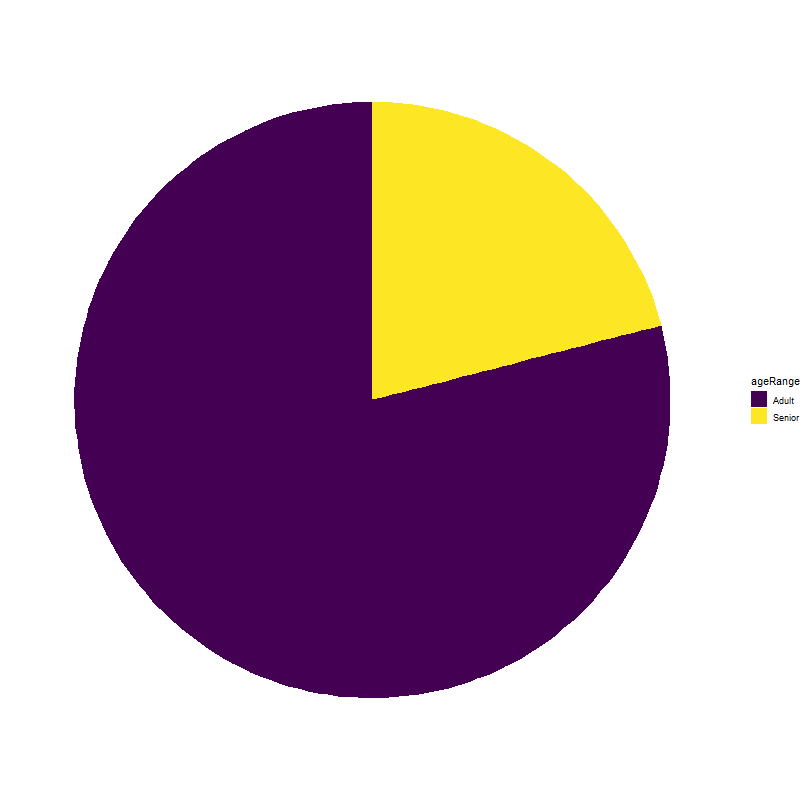
\includegraphics[width=.4\textwidth]{Img/EDA/EDA001.png}
    \caption{Age pie Chart}
\end{figure}

\begin{figure}[h!]
    \centering
    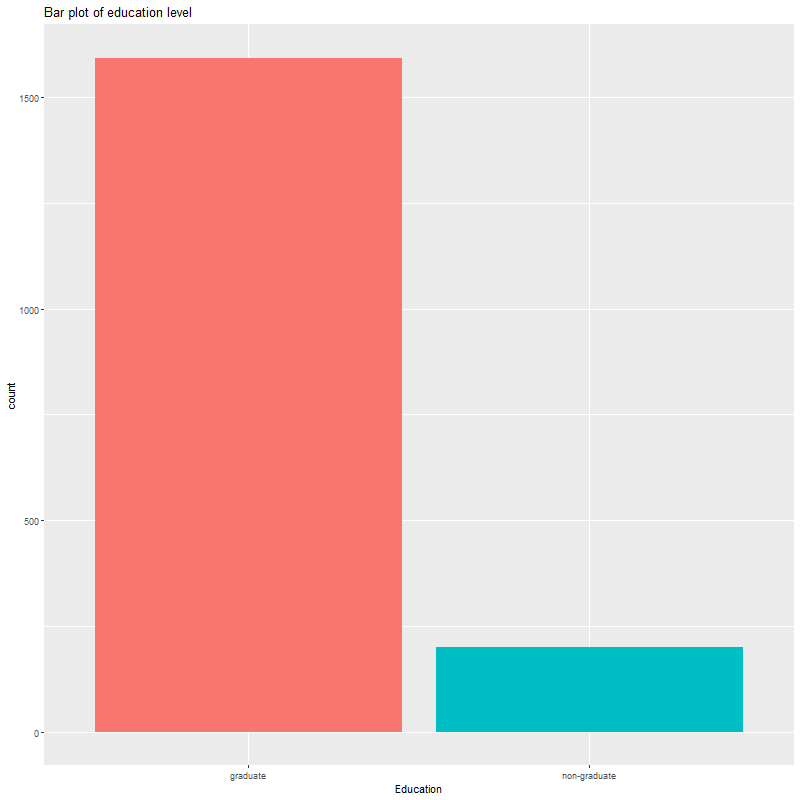
\includegraphics[width=.4\textwidth]{Img/EDA/EDA003.png}
    \caption{Education bar plot}
\end{figure}
\begin{figure}[h!]
    \centering
    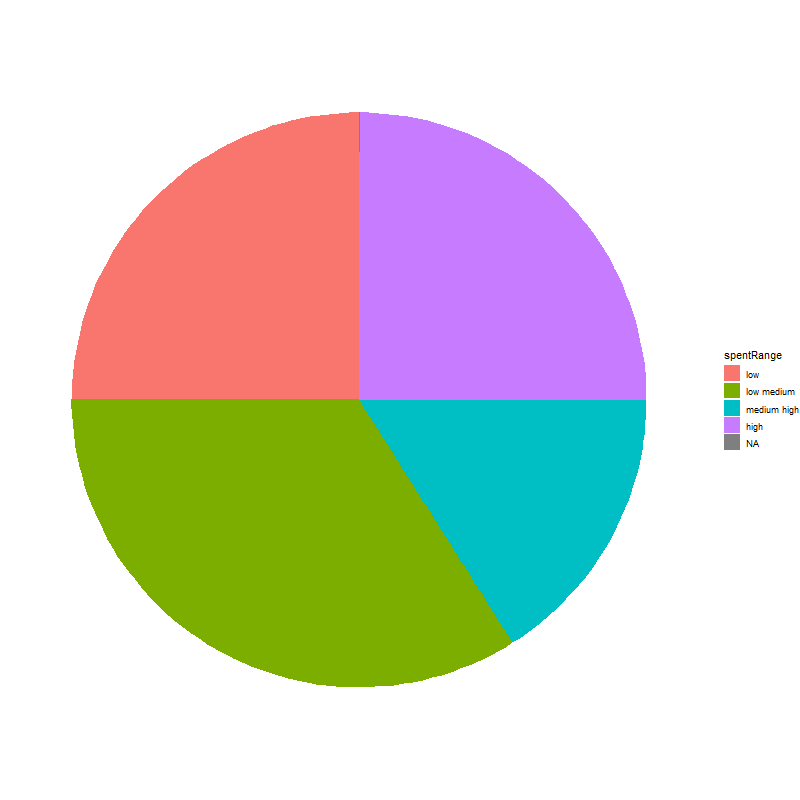
\includegraphics[width=0.4\textwidth]{Img/EDA/EDA004.png}
    \caption{Income pie Chart }
\end{figure}

\begin{figure}[h!]
    \centering
    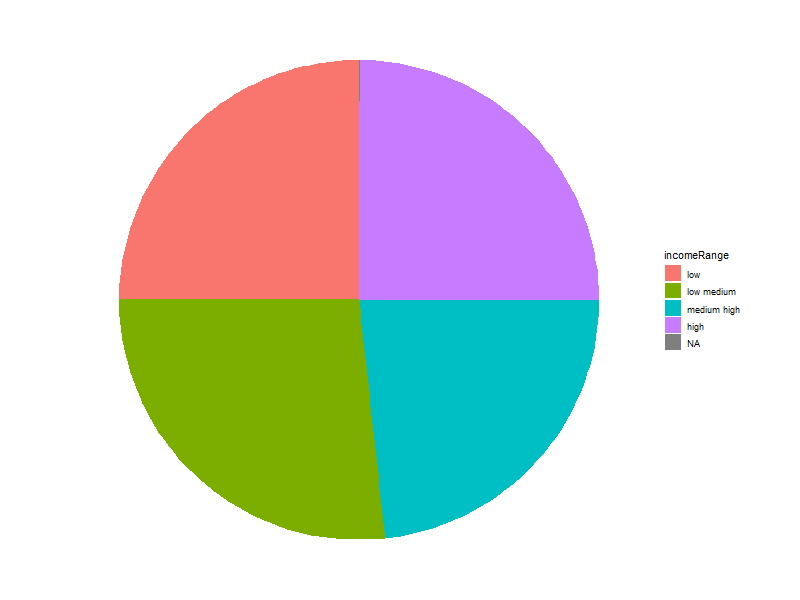
\includegraphics[width=.4\textwidth]{Img/EDA/EDA005.png}
    \caption{Total\_Spent pie Chart}
\end{figure}

Il primo grafico a torta è relativo alla variabile Age, il colore viola rappresenta il valore \textit{Adult} mentre il colore giallo \textit{Senior}. Dal grafico si ricava che la maggior parte degli individui è \textit{Adult}.
Il secondo rappresenta la variabile \textit{income}, il dataset è equi-distribuito in questo caso.
La distribuizione dei valori che assume la variabile \textit{Total spent} è raffigurata nella Figura 3. Da essa si ricava che low e high sono simili mentre quello più frequente è \textit{low medium}.\\
In seguito si sono seguite delle analisi per le variabili children, total spent e campaign.\\
La maggior parte delle istanze del dataset ha 1 figlio, la variabile Total\_Children è la somma tra la variabile KidHome e TeenHome. Questa informazione si è ricavata eseguendo il codice riportato i seguito.\\

\newpage
\subsubsection{Total Children}
Facendo il bar-plot della variabile \textit{Total\_Children} si nota che la maggior parte delle istanze presenti nel dataset ha 1 figlio.



\begin{figure}[h!]
    \centering
    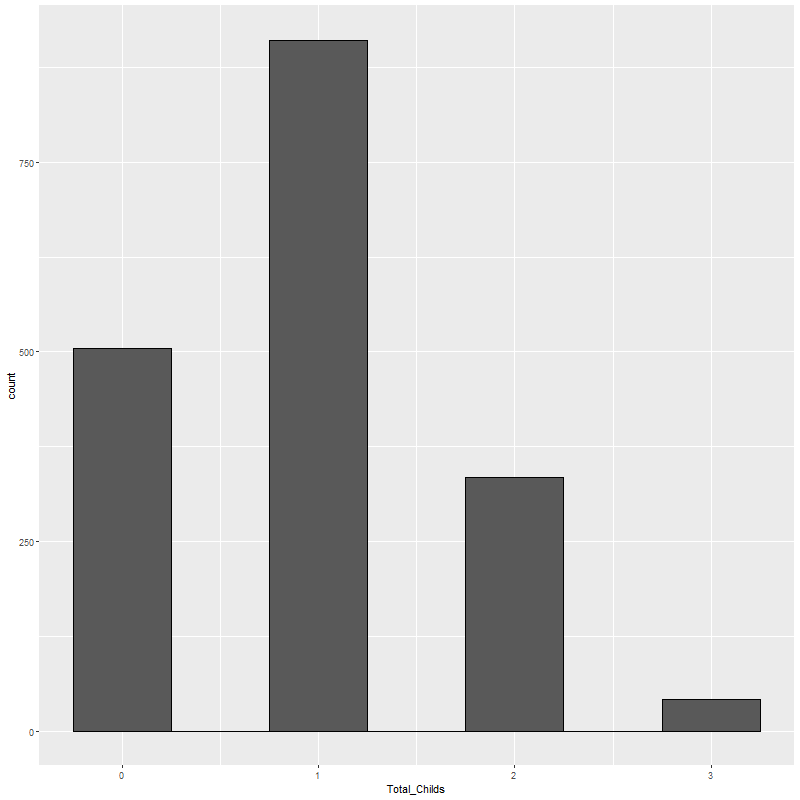
\includegraphics[width=.6\textwidth]{Img/EDA/EDA015.png}
    \caption{hist plot di total\_children }
\end{figure}

\newpage

\paragraph{Total\_Childen e Age}
Si è analizzata anche la relazione tra il numero totale di figli, \textit{Total\_children} ed \textit{Age} ed è risultato che tra gli \textit{Adult} il numero di figli più frequente è 1 e che rispetto ai \textit{Senior} hanno più figli.

\begin{lstlisting}[language=R]
age_children_histogram <- ggplot(trainingSet, aes(x=Total_Spent)) + geom_histogram(aes(fill=Age_range), binwidth = 0.5, colour = "Black")
age_children_histogram + facet_grid(Age_range~.)
\end{lstlisting}
\begin{figure}[h!]
    \centering
    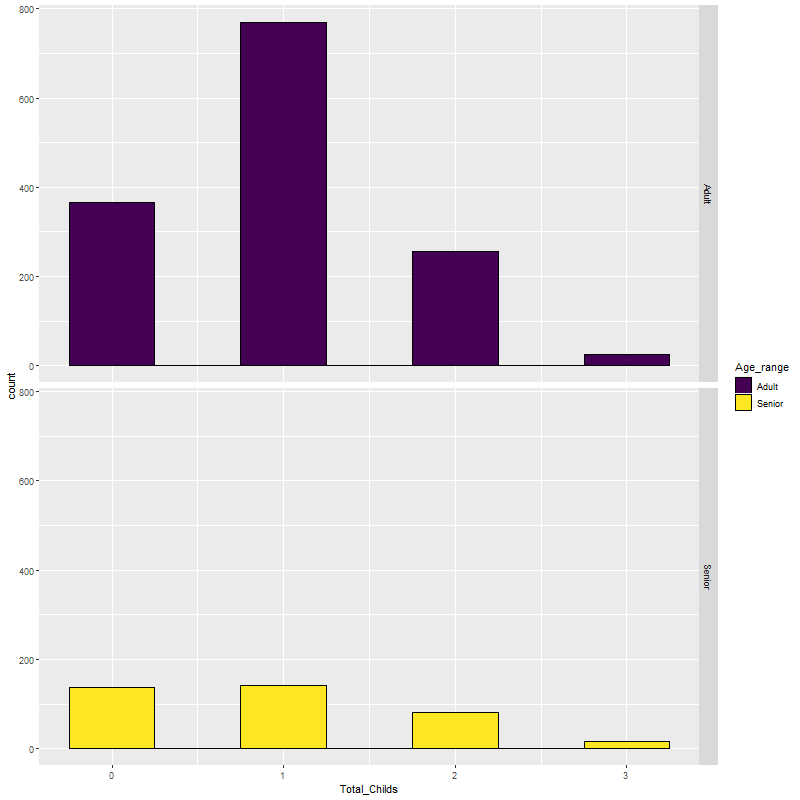
\includegraphics[width=.6\textwidth]{Img/EDA/EDA016.png}
    \caption{hist plot di Total\_Children e Age}
    \label{fig:fviz_eig(pca, addlabels = TRUE, ylim = c(0, 50))}
\end{figure}

\newpage

\paragraph{Total\_Children e Marital\_Status}
Nel pre processing i valori che può assumere la variabile \textit{Marital\_Status}sono stati collassati in due possibili valori.
\textit{Marital\_Status} è 0 se l'istanza ha come valore dell'attributo \textit{Marital\_Status} è \textit{single}, \textit{widow} oppure \textit{divorced}.
E' uguale a 1 se il valore assunto da \textit{Marital\_Status} è \textit{couple} oppure \textit{together}.
Rappresentando il diagramma a barre considerando \textit{Total\_Children}e \textit{Marital\_Status} si ricava che la maggior parte delle istanze ha un figlio. Il numero di istanze con \textit{Marital\_Status} pari a 0 è minore rispetto a quelle con valore uguale a 1 per i casi di zero e due figli, mentre per il caso di tre figli sono molto simili.


\begin{figure}[h!]
    \centering
    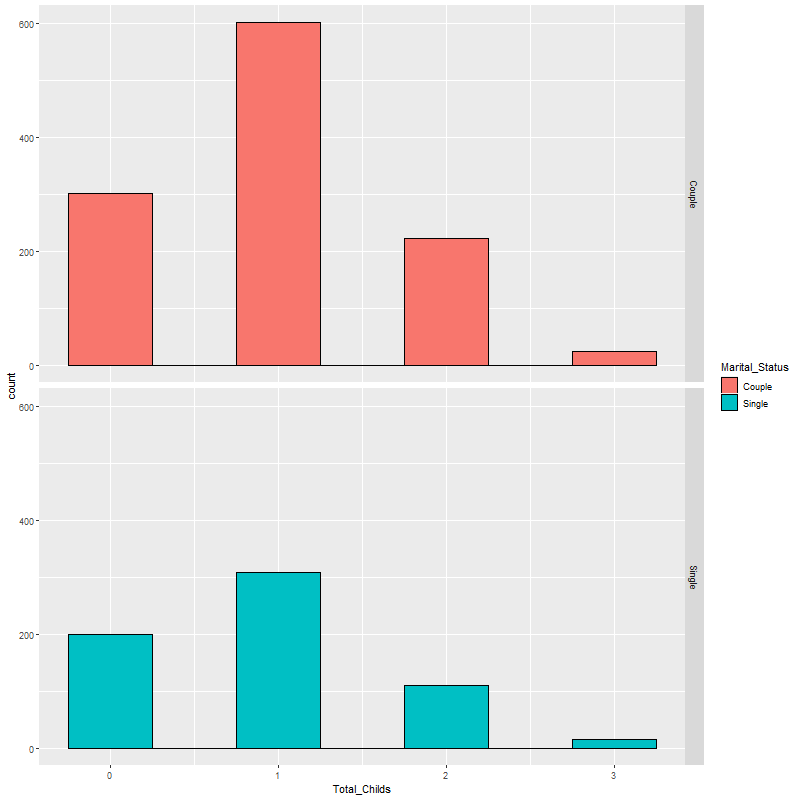
\includegraphics[width=.6\textwidth]{Img/EDA/EDA017.png}
    \caption{hist plot di Total\_Children e Marital\_Status}
    \label{fig:fviz_eig(pca, addlabels = TRUE, ylim = c(0, 50))}
\end{figure}

\newpage
\paragraph{Total\_Children e Education}

\begin{figure}[h!]
    \centering
    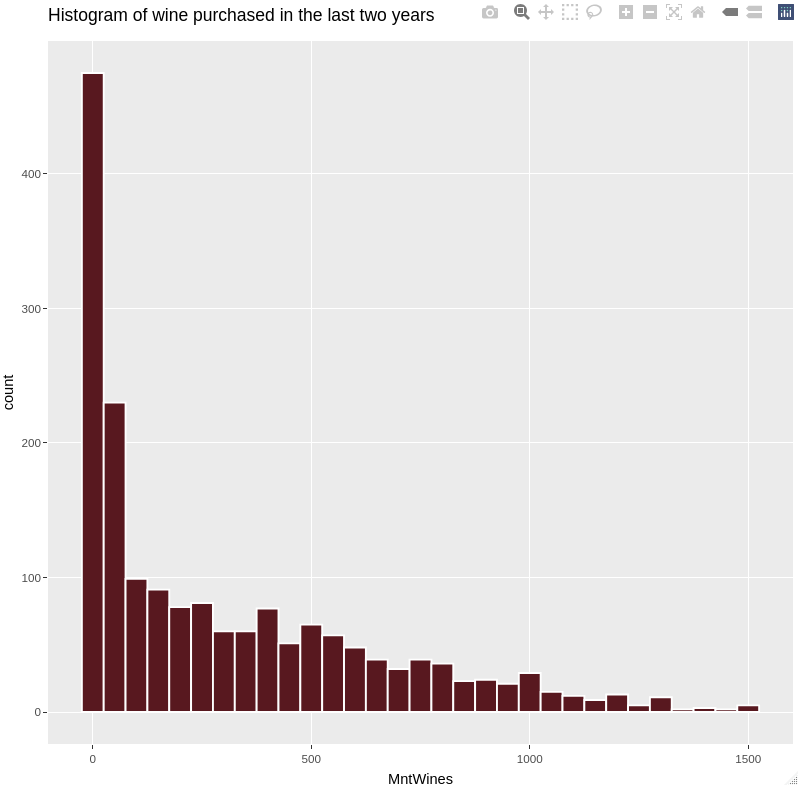
\includegraphics[width=.6\textwidth]{Img/EDA/EDA018.png}
    \caption{hist plot di Total\_Children e Education}
    \label{fig:fviz_eig(pca, addlabels = TRUE, ylim = c(0, 50))}
\end{figure}



\paragraph{Total\_Children e Income}

Sia dall' hist plot che dal jitte rplot si nota che più è basso il guadagno più si hanno figli. Nel caso di due figli ci sono più casi di persone con stipendio \textit{low medium} rispetto a chi ha uno stipendio \textit{low}. 
Nel caso di istanze con stipendio \textit{high} è comune che si abbiano figli. 


\begin{figure}[h!]
    \centering
    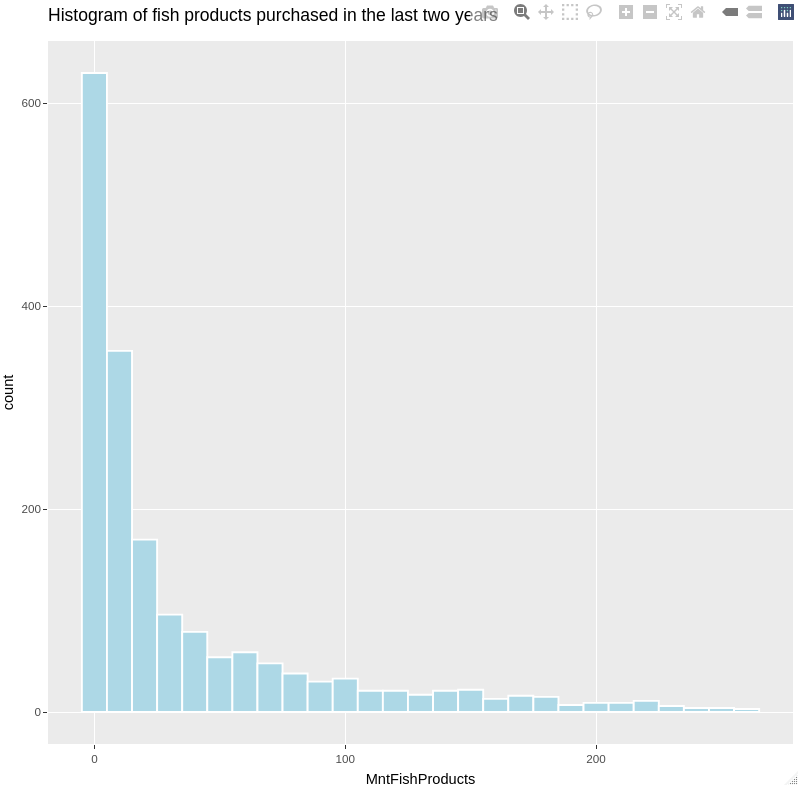
\includegraphics[width=0.5\textwidth]{Img/EDA/EDA021.png}
    \caption{jitter plot di Total\_Children e Income}
    \label{fig:fviz_eig(pca, addlabels = TRUE, ylim = c(0, 50))}
\end{figure}


\begin{figure}[h!]
    \centering
    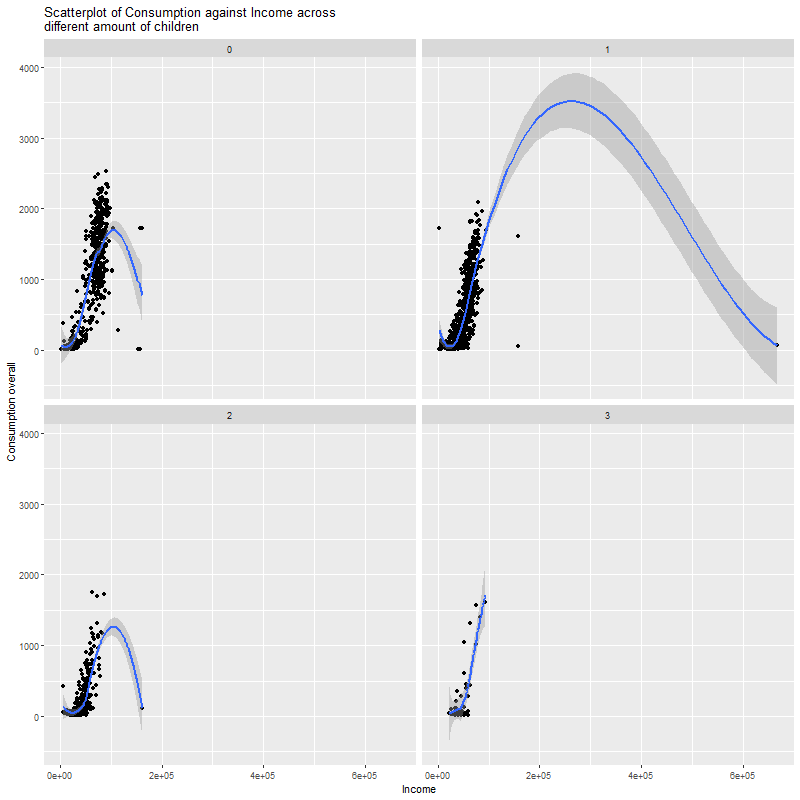
\includegraphics[width=0.5\textwidth]{Img/EDA/EDA022.png}
    \caption{scatter plot , Income e Total\_Children }
    \label{fig:fviz_eig(pca, addlabels = TRUE, ylim = c(0, 50))}
\end{figure}

\paragraph{Total\_Children jitter+boxplot}


\subsubsection{Total Spent}
La maggior parte degli individui spende meno di 500\$.

\begin{figure}[h!]
    \centering
    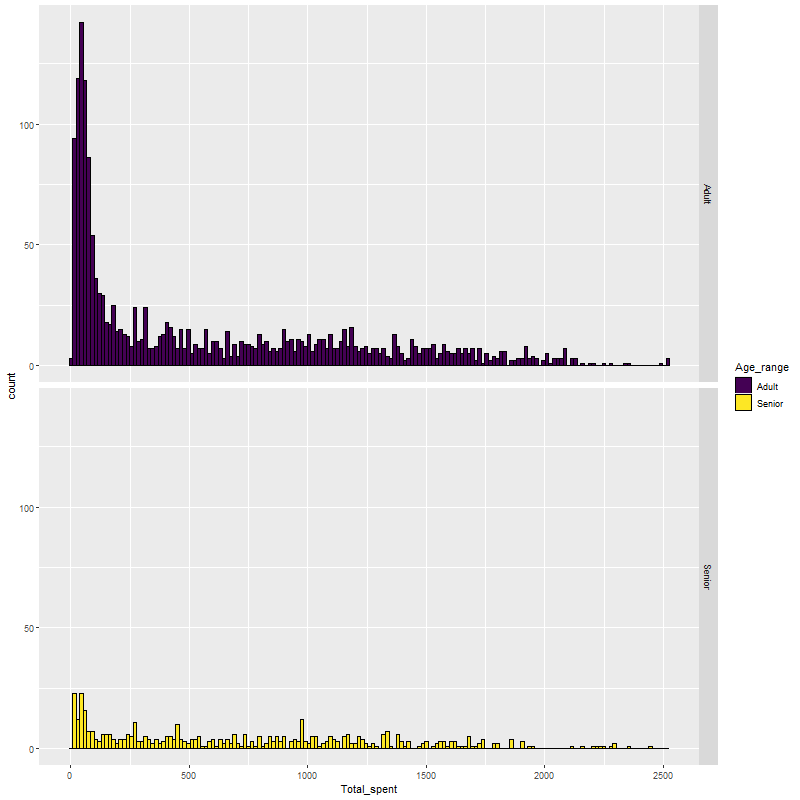
\includegraphics[width=.5\textwidth]{Img/EDA/EDA024.png}
    \caption{hist plot di total\_spent }
\end{figure}

Facendo il bar-plot della variabile \textit{Total\_Spent} si nota che le istanze presenti nel dataset spendono più per il vino e per la carne. 



\begin{figure}[h!]
    \centering
    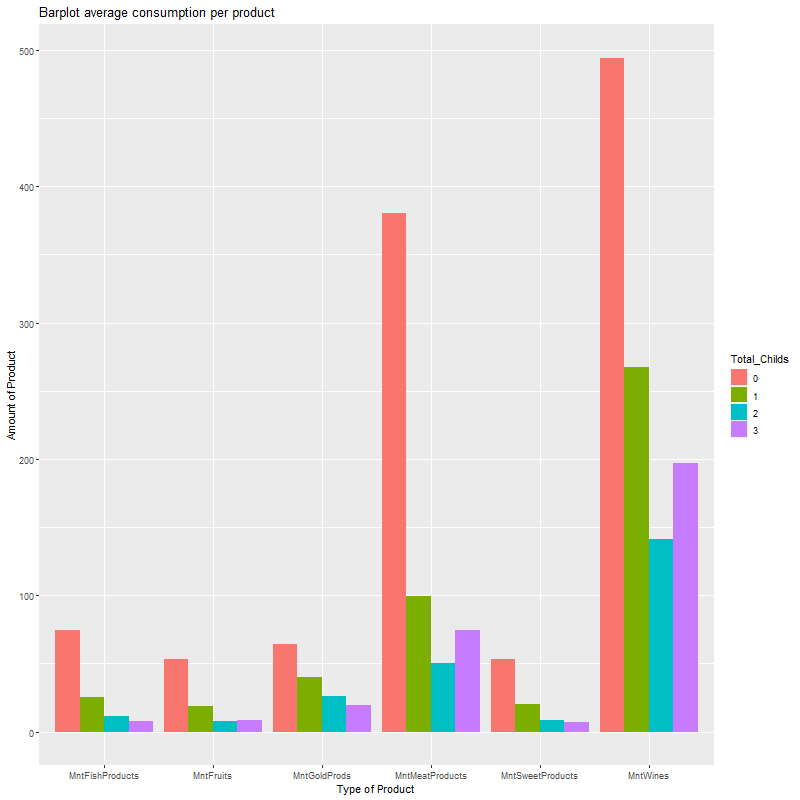
\includegraphics[width=.5\textwidth]{Img/EDA/EDA023.png}
    \caption{hist plot di total\_spent distinguedo tipi di prodotto }
\end{figure}

Per poter produrre il grafico della Figura 12 sono stati sommati i totali che ogni istanza ha speso per un certo prodotto.




\paragraph{Total Spent e Age}
La maggior parte degli individui spende meno di 500\$.


\begin{figure}[h!]
    \centering
    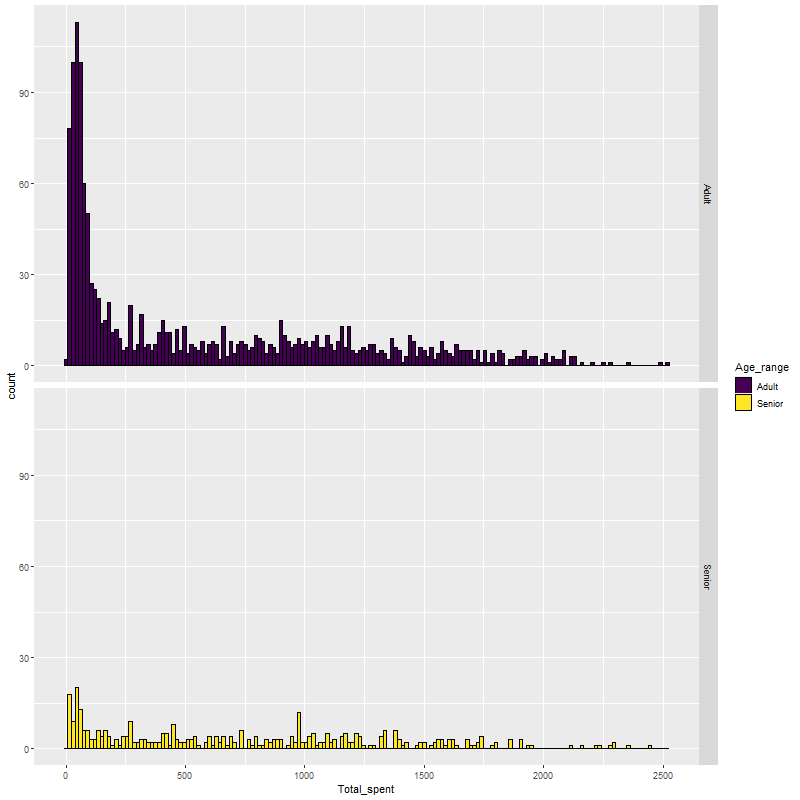
\includegraphics[width=.5\textwidth]{Img/EDA/EDA026.png}
    \caption{hist plot di Total\_Spent e Age }
\end{figure}


\begin{figure}[h!]
    \centering
    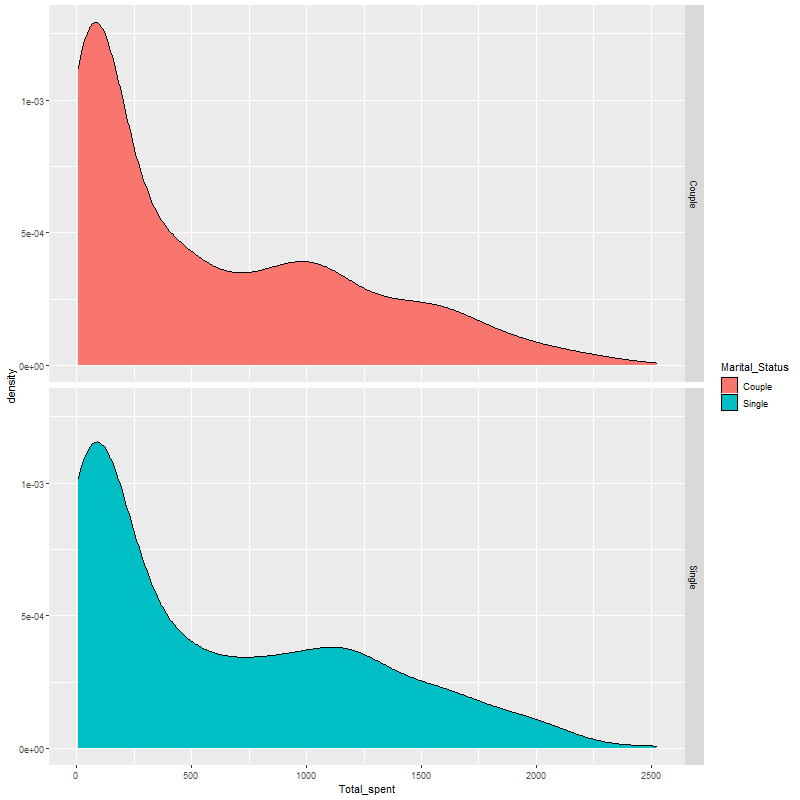
\includegraphics[width=.5\textwidth]{Img/EDA/EDA027.png}
    \caption{density plot di Total\_Spent e Age }
\end{figure}

\paragraph{Total Spent e Marital\_Status}
In questo caso sembrano simili. la maggior parte delle coppie spende un totale inferiore a 500.
La situazione in single è un po' più rilassata sarà che la maggior parte degli individui
 nel set di dati sono coppia



\begin{figure}[h!]
    \centering
    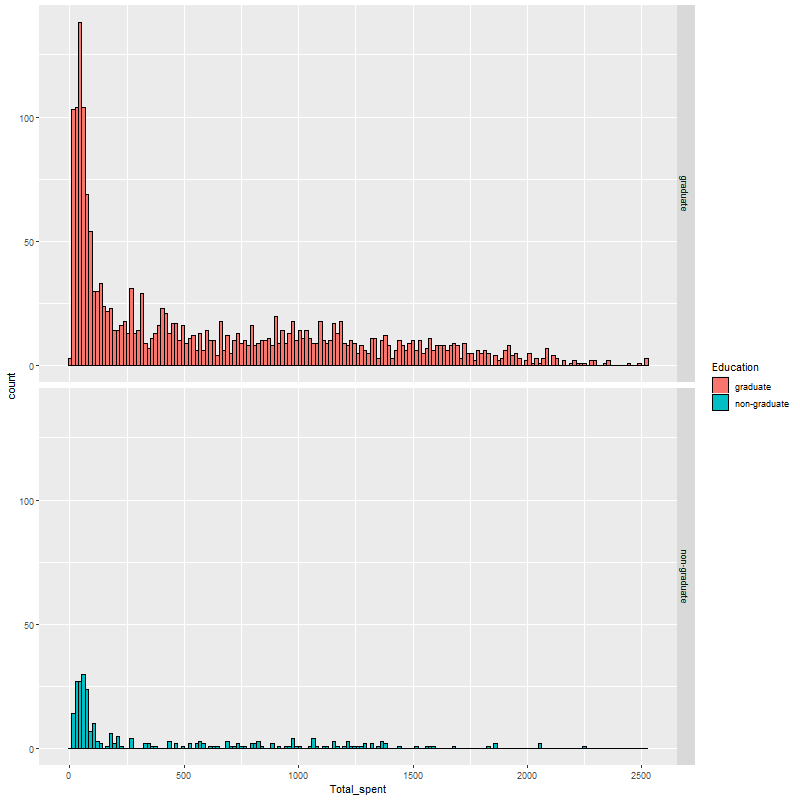
\includegraphics[width=.5\textwidth]{Img/EDA/EDA028.png}
    \caption{hist plot di Total\_Spent e Marital\_Status }
\end{figure}




\begin{figure}[h!]
    \centering
    \includegraphics[width=.5\textwidth]{Img/total spent analysis/density_plot/[DENSITY| TS] Marital_Status.png}
    \caption{density plot di Total\_Spent e Marital\_Status }
\end{figure}

\paragraph{Total Spent ed Education}
I laureati in genere spendono più dei non laureati. la maggior parte dei non laureati spende da 0 a 1500. da 1500 ci sono più casi di laureati che non laureati.

\begin{figure}[h!]
    \centering
    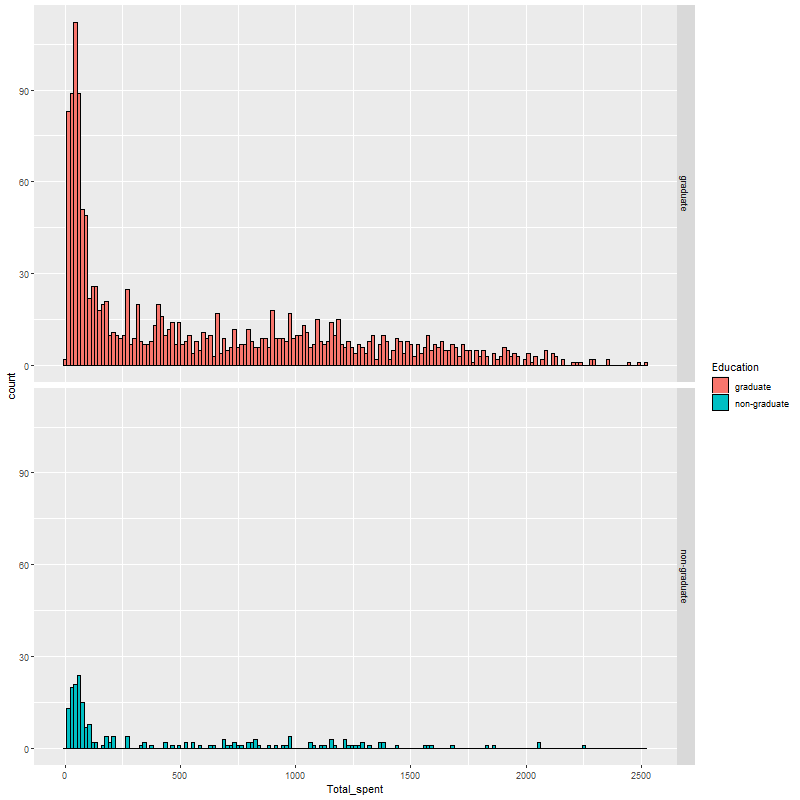
\includegraphics[width=.5\textwidth]{Img/EDA/EDA030.png}
    \caption{hist plot di Total\_Spent e Education}
\end{figure}


Il grafico della densità   è molto simile a quello della variabile \textit{Marital\_Status}.


\begin{figure}[h!]
    \centering
    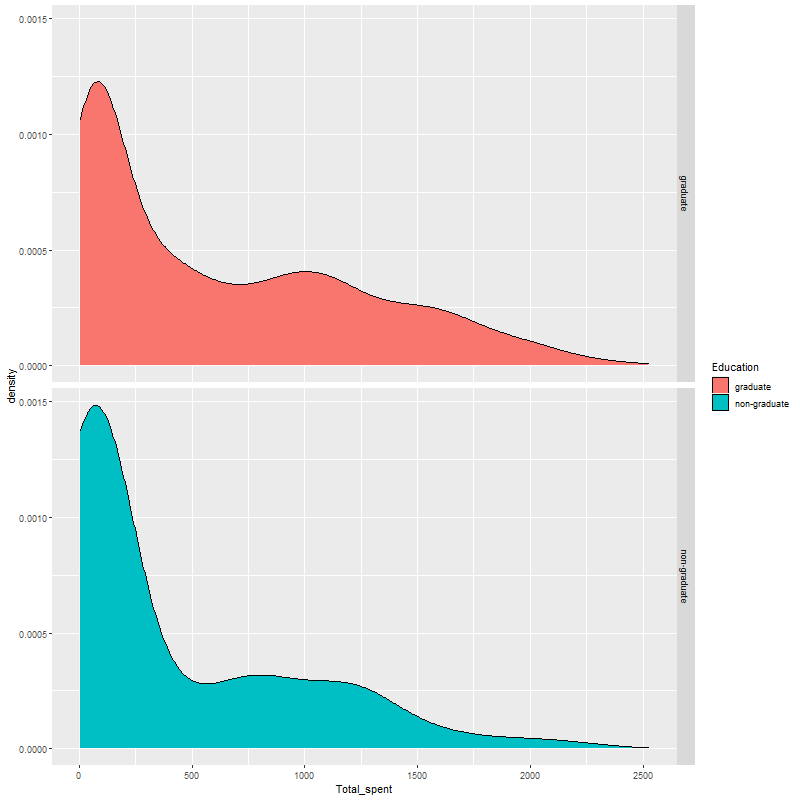
\includegraphics[width=.5\textwidth]{Img/EDA/EDA031.png}
    \caption{density plot di Total\_Spent e Education}
\end{figure}

\newpage

\paragraph{Total Spent e Total\_Children}



\begin{figure}[h!]
    \centering
    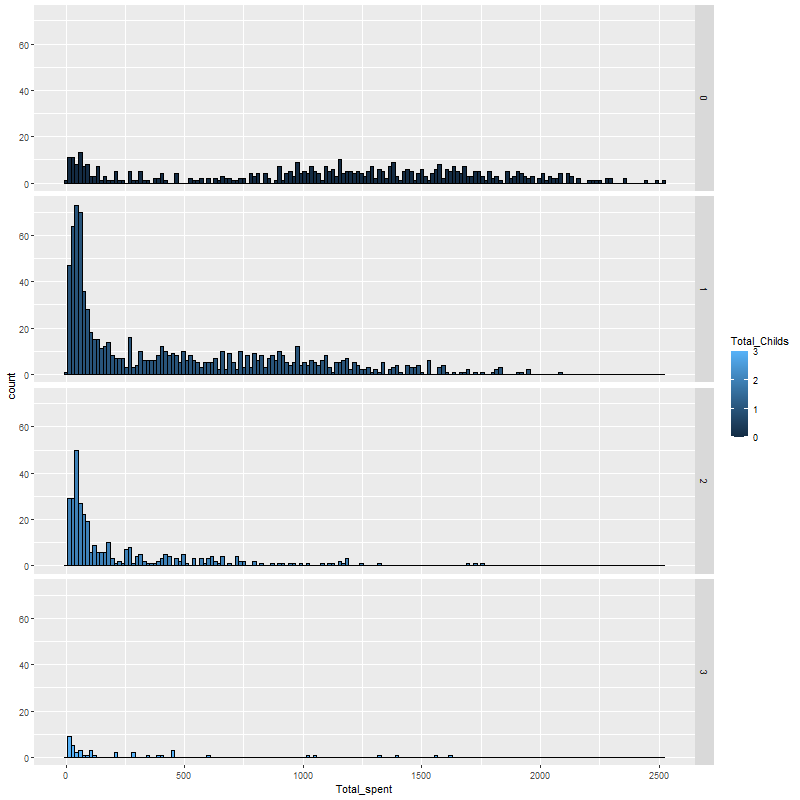
\includegraphics[width=.5\textwidth]{Img/EDA/EDA032.png}
    \caption{hist plot di Total\_Spent e Total\_Children}
\end{figure}


Di seguito il grafico della densità.



\begin{figure}[h!]
    \centering
    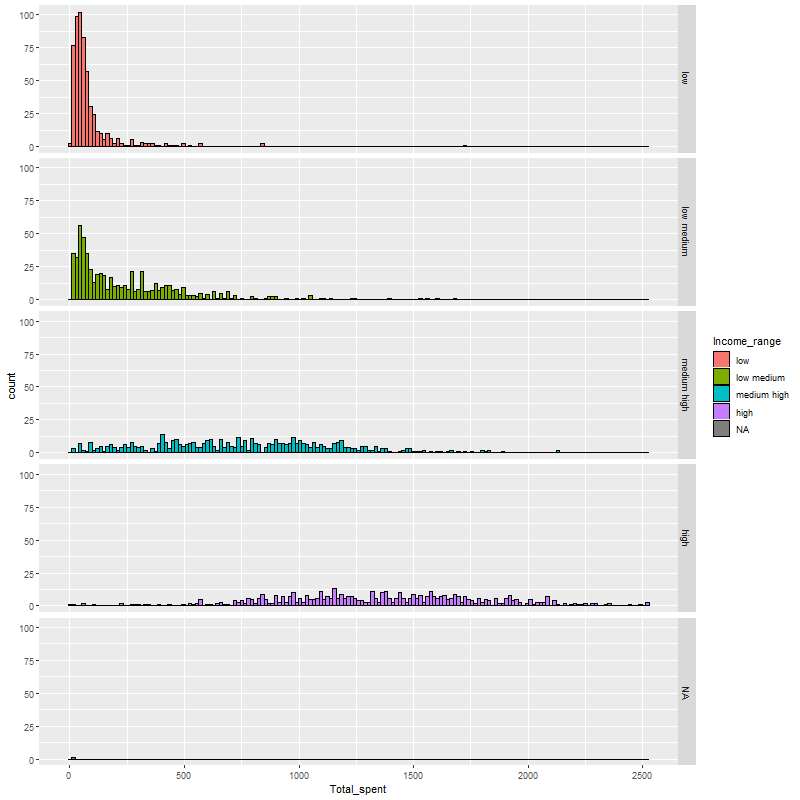
\includegraphics[width=.5\textwidth]{Img/EDA/EDA033.png}
    \caption{density plot di Total\_Spent e Total\_Children}
\end{figure}

\newpage
\paragraph{Total Spent e Income}



\begin{figure}[h!]
    \centering
    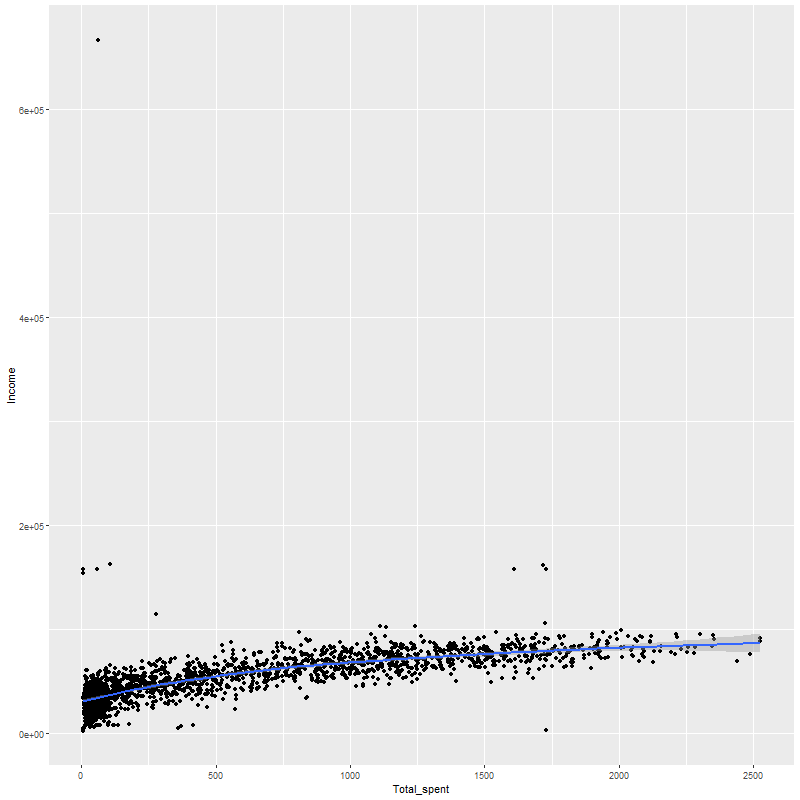
\includegraphics[width=.5\textwidth]{Img/EDA/EDA034.png}
    \caption{hist plot di Total\_Spent e Income}
\end{figure}



\begin{figure}[h!]
    \centering
    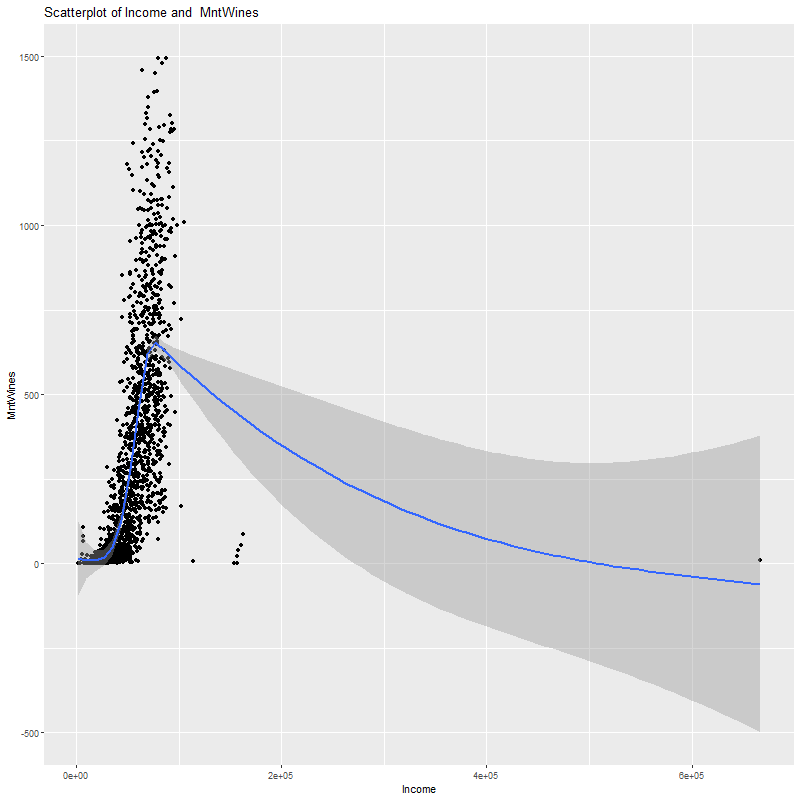
\includegraphics[width=.5\textwidth]{Img/EDA/EDA035.png}
    \caption{jitter plot di Total\_Spent e Income}
\end{figure}

\newpage

\paragraph{Total Spent jitter+boxplot}



\begin{figure}[h!]
    \centering
    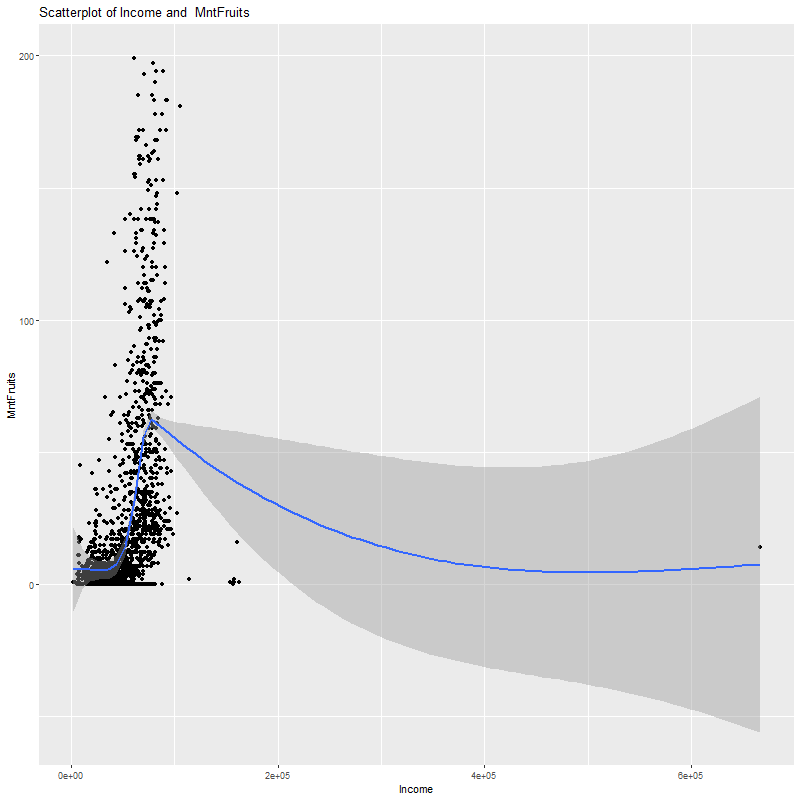
\includegraphics[width=.5\textwidth]{Img/EDA/EDA036.png}
    \caption{jitter boxplot di Total\_Spent, Income e Marital\_Status.}
\end{figure}



\begin{figure}[h!]
    \centering
    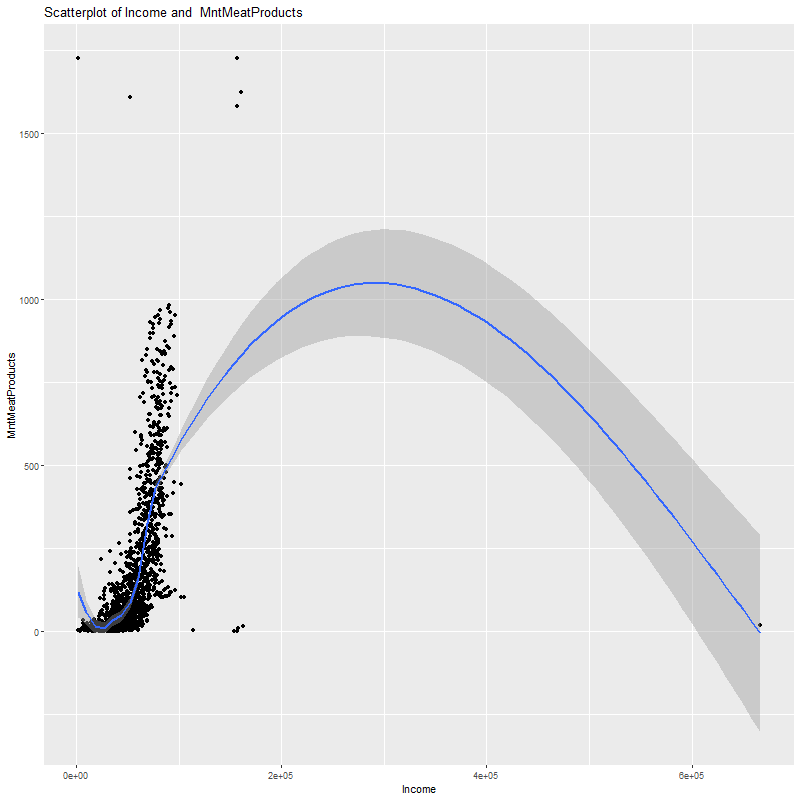
\includegraphics[width=.5\textwidth]{Img/EDA/EDA037.png}
    \caption{jitter boxplot di Total\_Spent, Income e Total\_Children.}
\end{figure}

\newpage



\begin{figure}[h!]
    \centering
    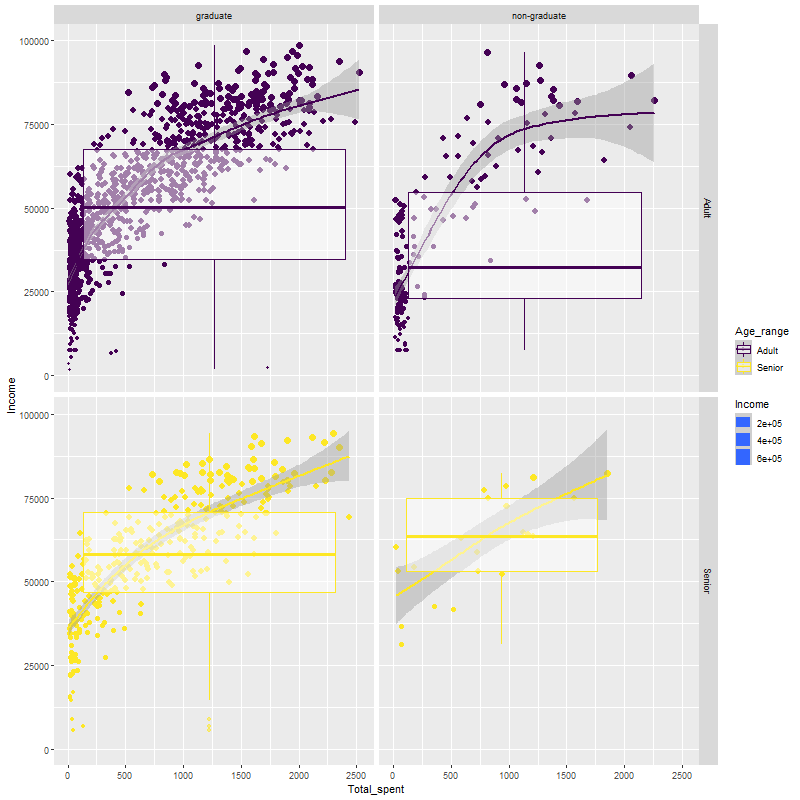
\includegraphics[width=.5\textwidth]{Img/EDA/EDA038.png}
    \caption{jitter boxplot di Total\_Spent, Income ed Age.}
\end{figure}

\newpage

\subsubsection{Campaign Analysis}
Si è eseguita un'analisi anche sulle campagne accettate da ogni individuo. 

\paragraph{Total\_Campaign}


\paragraph{Total Spent e Age}

\paragraph{Total Spent e Marital\_Status}

\paragraph{Total Spent ed Education}

\paragraph{Total Spent e Total\_Children}

\paragraph{Total Spent e Income}

\paragraph{Total Spent jitter+boxplot}

\newpage


\subsection{PCA}
La PCA è stata prevalentemente sfruttata al fine di ridurre il numero elevato di variabili che descrivono l'insieme di dati a un numero minore di variabili latenti, limitando il più possibile la perdita di informazioni. Il codice seguente mostra parte del codice riportato durante l'analisi dei dati.
\begin{lstlisting}[language=R]
pca <- PCA(trainingSet_scaled, graph = FALSE)

#Getting the variance of the first 9 new dimensions
pca$eig[,2][1:9]

#Getting the cummulative variance
pca$eig[,3][1:5]

#Getting the most correlated variables
dimdesc(pca, axes = 1:2)

# get eigenvalue
get_eigenvalue(pca)

# visualize pca
fviz_eig(pca, addlabels = TRUE, ylim = c(0, 50))
fviz_contrib(pca, choice = "var", axes = 1, top = 5)
fviz_pca_biplot(pca)

#Creating a factor map for the variable contributions
fviz_pca_var(pca, col.var = "contrib", repel = TRUE)

fviz_pca_var(pca, select.var = list(contrib = 5), col.var = "contrib", repel = TRUE)
\end{lstlisting}
Da esso si vuole dare particolare attenzione alla funzione \textit{get\_eigenvalue(pca)} che fornire le informazioni rappresentate nella tabella \ref{fig:get_eigenvalue(pca)}. Si vuole anche fornire un riferimento grafico a quest'ultima tramite l'output della funzione \textit{fviz\_eig(pca, addlabels = TRUE, ylim = c(0, 50))} descritto dalla figura \ref{fig:fviz_eig(pca, addlabels = TRUE, ylim = c(0, 50))}. Da essa si può notare che le prime 5 dimensioni fornite dalla PCA forniscono il 70\% della varianza cumulativa, per questo motivo si è deciso di prendere in considerazione tali dimensioni. Inoltre si vuole sottolineare l'importanza della prima dimensione che riesce a spiegare più del 40\% della varianza dei dati.
\begin{table}[h!t]
\centering
\begin{tabular}{rrrr}
  \hline
 & eigenvalue & variance.percent & cumulative.variance.percent \\ 
  \hline
Dim.1 & 6.98 & 41.06 & 41.06 \\ 
  Dim.2 & 1.75 & 10.32 & 51.38 \\ 
  Dim.3 & 1.15 & 6.78 & 58.16 \\ 
  Dim.4 & 1.05 & 6.19 & 64.35 \\ 
  Dim.5 & 1.00 & 5.87 & 70.22 \\ 
  Dim.6 & 0.79 & 4.66 & 74.88 \\ 
  Dim.7 & 0.66 & 3.91 & 78.79 \\ 
  Dim.8 & 0.63 & 3.70 & 82.49 \\ 
  Dim.9 & 0.57 & 3.33 & 85.82 \\ 
  Dim.10 & 0.47 & 2.77 & 88.59 \\ 
  Dim.11 & 0.42 & 2.49 & 91.08 \\ 
  Dim.12 & 0.39 & 2.30 & 93.38 \\ 
  Dim.13 & 0.35 & 2.05 & 95.43 \\ 
  Dim.14 & 0.31 & 1.81 & 97.24 \\ 
  Dim.15 & 0.25 & 1.46 & 98.69 \\ 
  Dim.16 & 0.22 & 1.31 & 100.00 \\ 
  Dim.17 & 0.00 & 0.00 & 100.00 \\ 
   \hline
\end{tabular}
\caption{Output funzione \textit{get\_eigenvalue(pca)}}
\label{fig:get_eigenvalue(pca)}
\end{table}
\begin{figure}[h!]
    \centering
    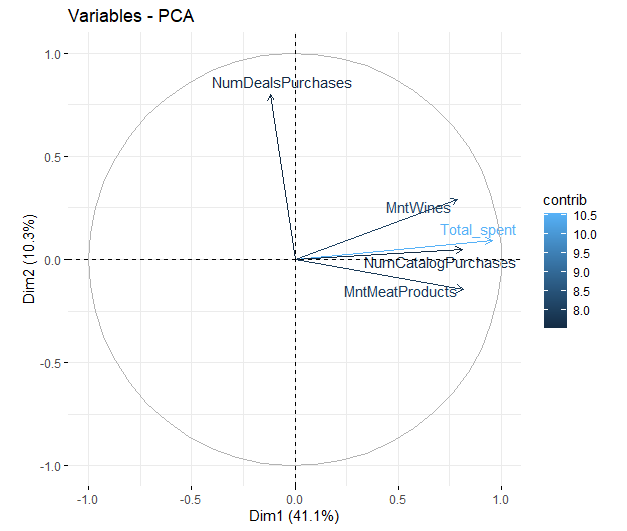
\includegraphics[width=0.7\textwidth]{Img/PCA/Rplot04.png}
    \caption{Output funzione \textit{fviz\_eig(pca, addlabels = TRUE, ylim = c(0, 50))}}
    \label{fig:fviz_eig(pca, addlabels = TRUE, ylim = c(0, 50))}
\end{figure}
In particolare la tabella \ref{fig:pca$var$contrib} vuole far notare il contributo di ciascun attributo del dataset nella creazione delle dimensioni della pca. Da essa possiamo notare le cinque principali variabili che hanno contribuito maggiormente nella creazione della prima dimensione della \textit{principal component analysis}: Total\_spent, MntMeatProducts, NumCatalogPurchases, MntWines e MntFishProducts. La figura \ref{fig:fviz_contrib(pca, choice = "var", axes = 1, top = 5)} ne mostra un grafico più esplicativo.
\begin{figure}[h!]
    \centering
    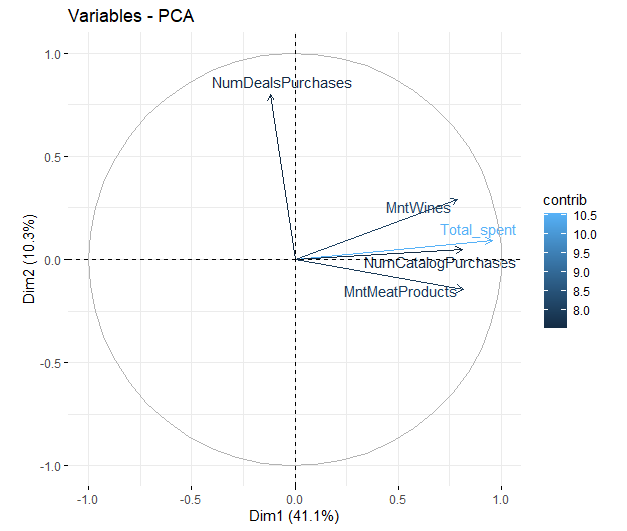
\includegraphics[width=0.7\textwidth]{Img/PCA/Rplot04.png}
    \caption{Output funzione \textit{fviz\_contrib(pca, choice = "var", axes = 1, top = 5)}}
    \label{fig:fviz_contrib(pca, choice = "var", axes = 1, top = 5)}
\end{figure}
\begin{table}[h!t]
\centering
\begin{tabular}{rrrrrr}
  \hline
 & Dim.1 & Dim.2 & Dim.3 & Dim.4 & Dim.5 \\ 
  \hline
Income & 7.31 & 0.16 & 2.59 & 3.75 & 0.92 \\ 
  Recency & 0.00 & 0.01 & 1.24 & 9.79 & 87.66 \\ 
  MntWines & 8.89 & 4.77 & 9.07 & 1.61 & 0.88 \\ 
  MntFruits & 6.99 & 1.23 & 11.85 & 0.00 & 0.35 \\ 
  MntMeatProducts & 9.55 & 1.20 & 0.11 & 0.00 & 0.12 \\ 
  MntFishProducts & 7.56 & 1.32 & 8.51 & 0.16 & 0.33 \\ 
  MntSweetProducts & 6.94 & 0.87 & 9.33 & 0.06 & 0.15 \\ 
  MntGoldProds & 4.69 & 2.38 & 6.52 & 1.19 & 0.31 \\ 
  NumDealsPurchases & 0.21 & 36.53 & 3.87 & 0.16 & 0.01 \\ 
  NumWebPurchases & 4.30 & 17.88 & 0.97 & 2.21 & 0.00 \\ 
  NumCatalogPurchases & 9.43 & 0.13 & 0.70 & 0.20 & 0.23 \\ 
  NumStorePurchases & 7.53 & 4.02 & 0.50 & 0.32 & 0.37 \\ 
  NumWebVisitsMonth & 5.78 & 8.73 & 0.35 & 12.79 & 1.36 \\ 
  Total\_spent & 13.06 & 0.49 & 0.82 & 0.58 & 0.34 \\ 
  Total\_Campains & 2.68 & 0.01 & 35.64 & 12.53 & 3.01 \\ 
  Total\_Childs & 4.79 & 14.87 & 0.20 & 2.76 & 0.15 \\ 
  Age & 0.28 & 5.40 & 7.71 & 51.88 & 3.81 \\ 
   \hline
\end{tabular}
\caption{Output \textit{pca\$var\$contrib}}
\label{fig:pca$var$contrib}
\end{table}
Le funzioni \textit{fviz\_pca\_var} hanno permesso di analizzare graficamente le dimensioni che spie

\section{Modelli utilizzati}
TODO
\subsection{K-Means}
TODO

\section{Esperimenti}
TODO

\subsection{Analisi dei risultati ottenuti}

\section{Conclusion}


\appendix

\section*{Appendix: }



\end{document}
